\documentclass[hyperref={pdfpagelabels=false}]{beamer}
% beamer already loads hyperref; do NOT load \usepackage{hyperref} again.

\usepackage{ragged2e} % 文字向兩邊對齊
\renewcommand{\raggedright}{\leftskip=0pt \rightskip=0pt plus 0cm}

\usepackage{listings}
\usepackage{lmodern}
\usepackage{fontspec}
\usepackage{xeCJK}
\setCJKmainfont{Noto Sans CJK TC}
%（可選）若你會用到無襯線中文或等寬中文，建議補上：
\setCJKsansfont{Noto Sans CJK TC}
\setCJKmonofont{Noto Sans Mono CJK TC}

\usepackage[english]{babel}
\usepackage{amsmath,amssymb,amsfonts,amsthm}

% hyperref settings (since beamer already loads hyperref)
\hypersetup{
  colorlinks=true,
  urlcolor=blue,
  citecolor=blue,
  pdfborder={0 0 0}
}

\usepackage{accsupp}% http://ctan.org/pkg/accsupp
\newcommand{\emptyaccsupp}[1]{\BeginAccSupp{ActualText={}}#1\EndAccSupp{}}

\usepackage{tikz}
\usetikzlibrary{arrows,decorations.pathmorphing,backgrounds,fit,positioning,shapes.symbols,chains}

\usepackage{booktabs}
\usepackage{threeparttable}
\usepackage{colortbl} 
\usepackage{xcolor}
\usetikzlibrary{tikzmark}

\newcommand{\indep}{\perp\!\!\!\perp}
\newcommand{\nindep}{\not\!\perp\!\!\!\perp}

\beamertemplatefootpagenumber


\usepackage{listings}
%%%%%%%%%%%%%%%%%%%%%%%%%%%%%%%%%%%%%%%%%%%%%%%%%%%%%%%%%%%%%%%%%%%%%%%%%%%%%%
% LaTeX snippet: language and style definition of Stata for listings package.
%                [listings](http://www.ctan.org/pkg/listings) 
%                [Stata](http://www.stata.com/)
%
% Usage:
%     Copy the code into your preamble, or import it by `\include` .
%     then in your doc:
%     \lstinputlisting[style=numbers]{DO-SCRIPT}
%     \lstinputlisting[style=numbers, style=stata-editor]{DO-SCRIPT}
%     \lstinputlisting[style=nonumbers, frame=none]{DO-SCRIPT}
% How it works:
%     - The language is defined by `\lstdefinelanguage{Stata}`
%     - Four styles is defined by `\lstdefinestyle{STYLE-NAME}`, 
%       they are: numbers and no numbers, plain(black and white) and colorful
%       (colored roughly like stata editor.)
% Tips:
%     - Generally you only need to set your default in the last part,
%       that is, code inside of `\lstset`.
%     - Add more keywords(I can not list all of them) in the `\lstset` part.
%     - Do NOT leave any blank lines in commands
%       (`\lstddefinelanguage', `\lstdefinestyle` and `\lstset`)
%
% update: 2014-04-16
% version: 0.1
% author: kongs
% licence: MIT
% url: https://gist.github.com/kongs-sublime/10862838
%
% TODO: 
%       - finish keyword list.
%       - precise colors that match stata editor?
%       - make it flexible(fonts and style)
%
%%%%%%%%%%%%%%%%%%%%%%%%%%%%%%%%%%%%%%%%%%%%%%%%%%%%%%%%%%%%%%%%%%%%%%%%%%%%%%


% langugae defination
\lstdefinelanguage{Stata}{
	% Left for users to add missing commands,
	% with possibility of choosing different style.
	morekeywords=,
	% Popular add-on commands
	morekeywords=[2]{cntrade, chinafin, 
		wbopendata, spmap,
	},
	% System commands
	morekeywords=[3]{regress, summarize, 
		display,
	},
	% Keywords
	morekeywords=[4]{forvalues, if, foreach, set},
	% Built-in functions
	morekeywords=[5]{rnormal, runiform},
	morecomment=[l]{//},
	% morecomment=[l]{*},  // `*` maybe used as multiply operator. So use `//` as line comment.
	morecomment=[s]{/*}{*/},
	% morecomment=[s]{,}{//},
	% The following is used by macros, like `lags'.
	morecomment=[n][keywordstyle9]{`}{'},
	morestring=[b]",
	sensitive=true,
}

\lstdefinestyle{numbers}{
	numbers=left, 
	stepnumber=1, 
	numberstyle=\tiny\emptyaccsupp,
	xleftmargin=2em,
}

\lstdefinestyle{nonumbers}{
	numbers=none,
}

\lstdefinestyle{stata-plain}{
	language=Stata,
	basicstyle=\footnotesize\ttfamily,
}

\lstdefinestyle{stata-editor}{
	language=Stata,
	basicstyle=\footnotesize\ttfamily,  
	keywordstyle={\color{NavyBlue}},  
	keywordstyle=[2]{\color{NavyBlue}},
	keywordstyle=[3]{\color{NavyBlue}},
	keywordstyle=[4]{\color{NavyBlue}},
	keywordstyle=[5]{\color{Blue}},
	keywordstyle=[9]{\color{TealBlue}},
	stringstyle=\color{Maroon},
	commentstyle=\color{OliveGreen},
}

\lstset{
	language=Stata,
	style=stata-plain,
	% style=stata-editor,
	style=numbers,
	showstringspaces=false,
	breaklines,
	frame=single,
	% To add missing commands
	% morekeywords={xtreg, xtunitroot},
}




\title[]  
{Synthetic Control Method}


\author 
{Prof. Tzu-Ting Yang  \\ 楊子霆}

%\institute{Institute of Economics, Academia Sinica  \\ Econ, NTU}
\institute{Institute of Economics, Academia Sinica  \\ 中央研究院經濟研究所}
%\institute{Institute of Economics, Academia Sinica  \\ Econ, NTU}
%\institute{Institute of Economics, Academia Sinica  \\ IMES/IDAS, NCCU}

%\author 
%{楊子霆 \\ 中研院經濟所}

%\institute 
%{中正大學國際經濟專題研討}


\date
{\today}




% \usetheme{CambridgeUS}
% %\usecolortheme{seahorse}
% \setbeamertemplate{footline}{%
% 	\hfill\usebeamercolor[fg]{page number in head/foot}%
% 	\usebeamerfont{page number in head/foot}%
% 	\insertframenumber\,/\,\inserttotalframenumber\hspace{1em}\vspace{2pt}%
% }

% \usetheme{Boadilla}
% %\useinnertheme{rectangles}

% %\usetheme{CambridgeUS}
% \usecolortheme{seahorse}
% \setbeamertemplate{footline}{%
% 	\hfill\usebeamercolor[fg]{page number in head/foot}%
% 	\usebeamerfont{page number in head/foot}%
% 	\insertframenumber\,/\,\inserttotalframenumber\hspace{1em}\vspace{2pt}%
% }


%\usepackage{beamerthemeshadow}
%\usecolortheme{seahorse}
\setbeamertemplate{footline}{%
	\hfill\usebeamercolor[fg]{page number in head/foot}%
	\usebeamerfont{page number in head/foot}%
	\insertframenumber\,/\,\inserttotalframenumber\hspace{1em}\vspace{2pt}%
}


%\usepackage{beamerthemeshadow}

\beamersetuncovermixins{\opaqueness<1>{25}}{\opaqueness<2->{15}}
\begin{document}
	
	
	\begin{frame}{}
	\titlepage
\end{frame}




\title[]  
{Main Idea}


\author 
{}

%\institute{Institute of Economics, Academia Sinica  \\ Econ, NTU}
%\institute{Institute of Economics, Academia Sinica  \\ IMES/IDAS, NCCU}
\institute{}

%\author 
%{楊子霆 \\ 中研院經濟所}

%\institute 
%{中正大學國際經濟專題研討}




\date
{}


\begin{frame}{}
	\titlepage
\end{frame}





%\begin{frame}{Synthetic Control Method}{Main Idea}
%	\begin{itemize}
%		\item SC is quite popular in social science due to the following features:	
%		\begin{itemize}
%			\vspace{0.2cm}
%			\item[1] It can evaluate treatment effects on \textbf{one (or very few) treated unit}
%			\vspace{0.2cm}
%			\begin{itemize}
%				\item Aggregate outcomes (e.g. county-level crime rate)
%			\end{itemize}
%			\vspace{0.2cm}
%			\item[2] Use a \textbf{data-driven procedure} and \textbf{a small number of non-treated units} to build the suitable counterfactuals		
%			
%			
%		\end{itemize}
%		
%		
%	\end{itemize}
%\end{frame}


\begin{frame}{Synthetic Control Method}{Main Idea}
\begin{itemize}
	\item Synthetic Control (SC) is a method to evaluate the causal effect of treatment.
\vspace{0.2cm}
\begin{itemize}
	\item Use (long) panel data to build the \textbf{weighted average of non-treated units} 
\vspace{0.2cm}
\begin{itemize}	
		\item The \textbf{weighted average of
		non-treated units} is the \textbf{synthetic unit}
	\vspace{0.2cm}
	\item Synthetic unit can best reproduce characteristics of the
	\textbf{treated unit} over time in pre-treatment period
	\vspace{0.2cm}
\end{itemize}

\item Causal effect of treatment can be quantified by a simple difference in the post-treatment period:
	\vspace{0.2cm}
\begin{itemize}		
\item \textbf{treated unit vs synthetic unit}
\end{itemize}
\end{itemize}
\end{itemize}
\end{frame}



\begin{frame}{Synthetic Control Method}{Graphical Representation}
\begin{center}
\begin{figure}[p]
\centering
%\scalebox{0.98}{\includegraphics{did_1.jpg}}
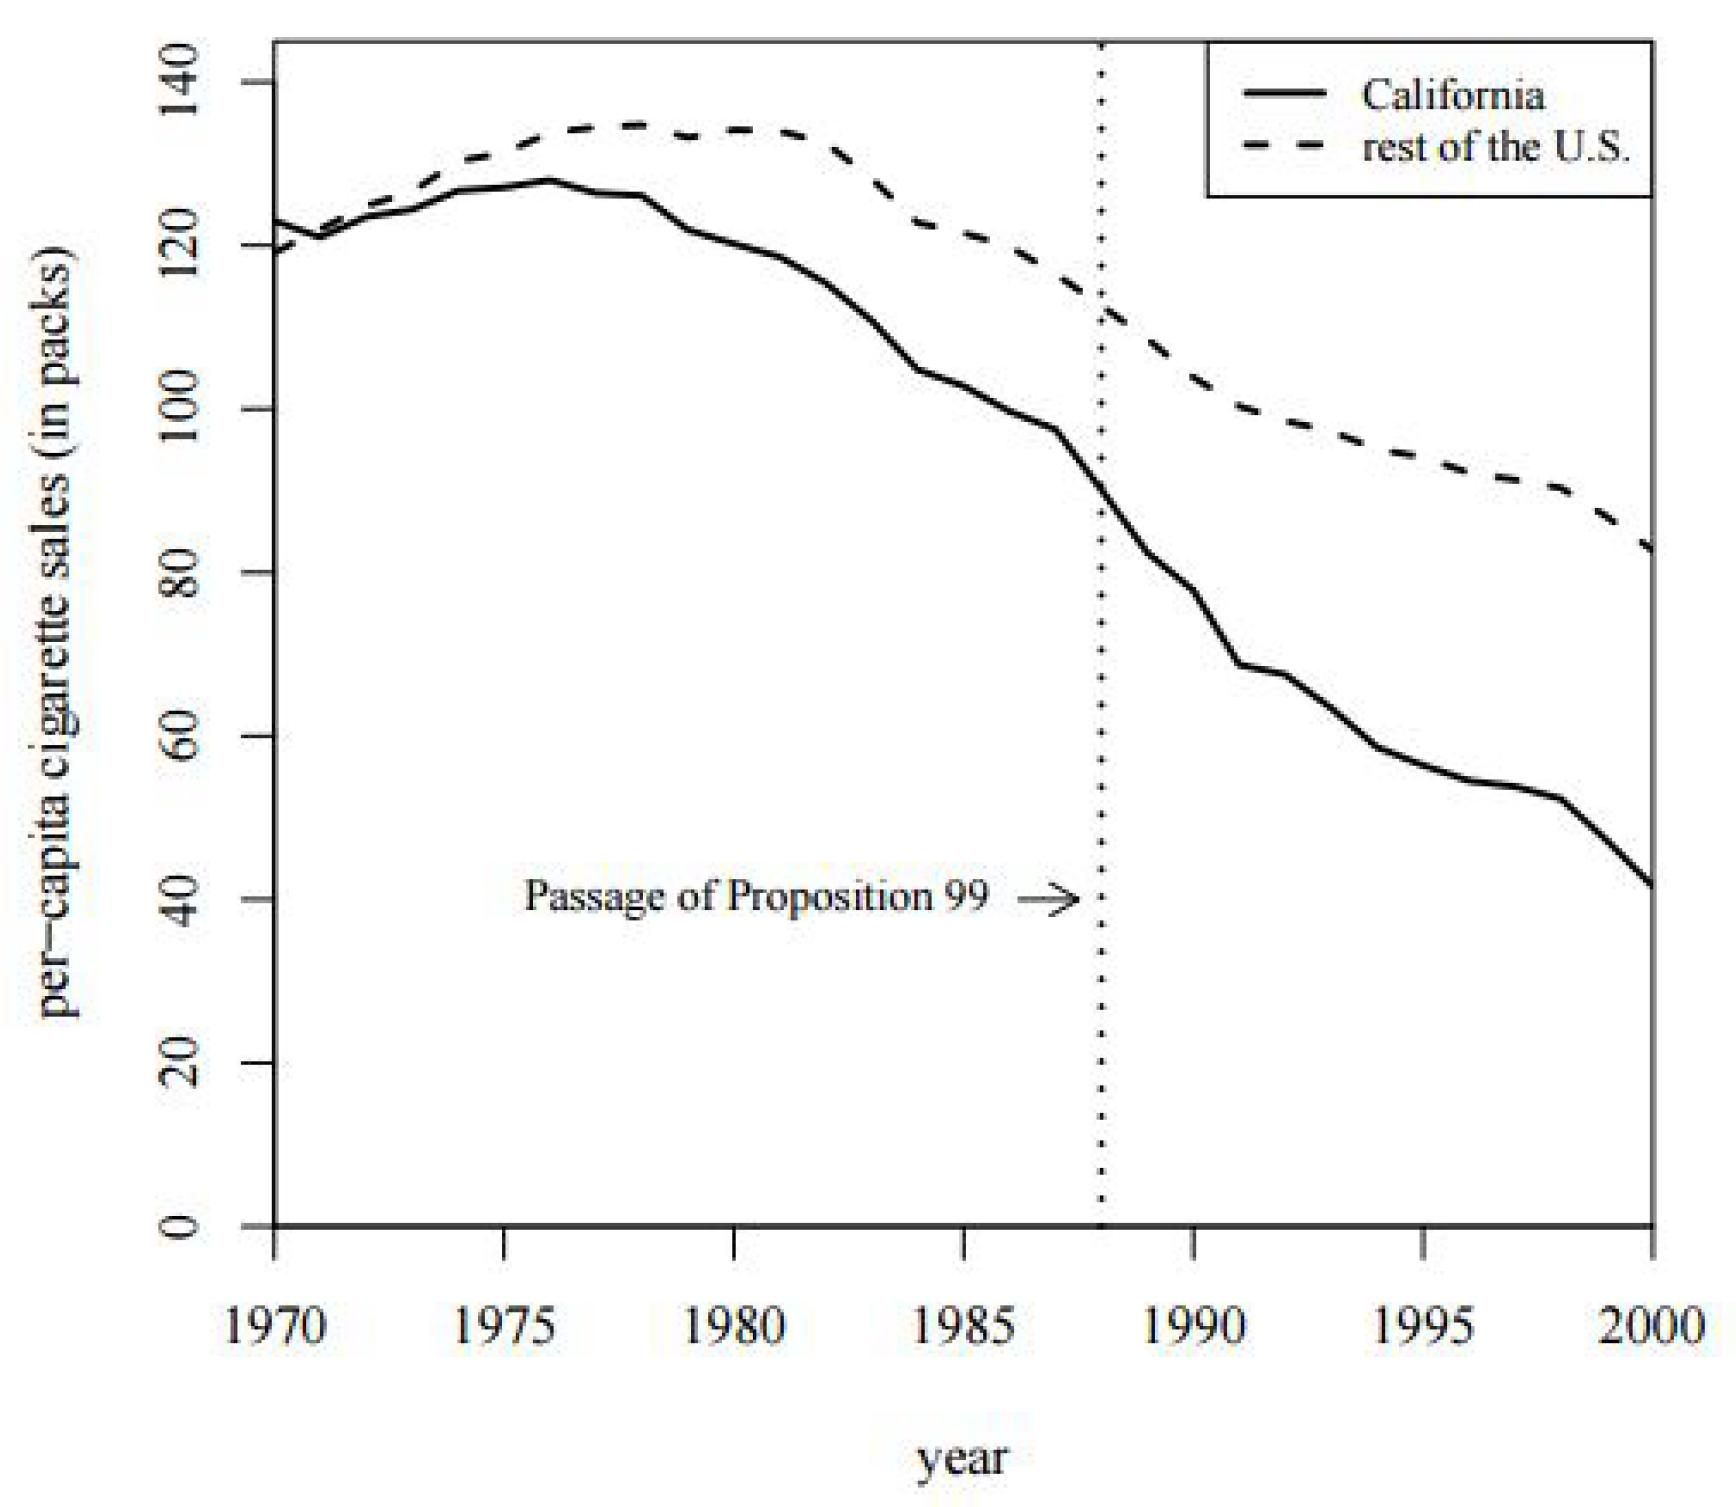
\includegraphics{figure/sc-2.jpg}
\end{figure}
\end{center}
\end{frame}


\begin{frame}{Synthetic Control Method}{Graphical Representation}
\begin{center}
\begin{figure}[p]
\centering
%\scalebox{0.98}{\includegraphics{did_1.jpg}}
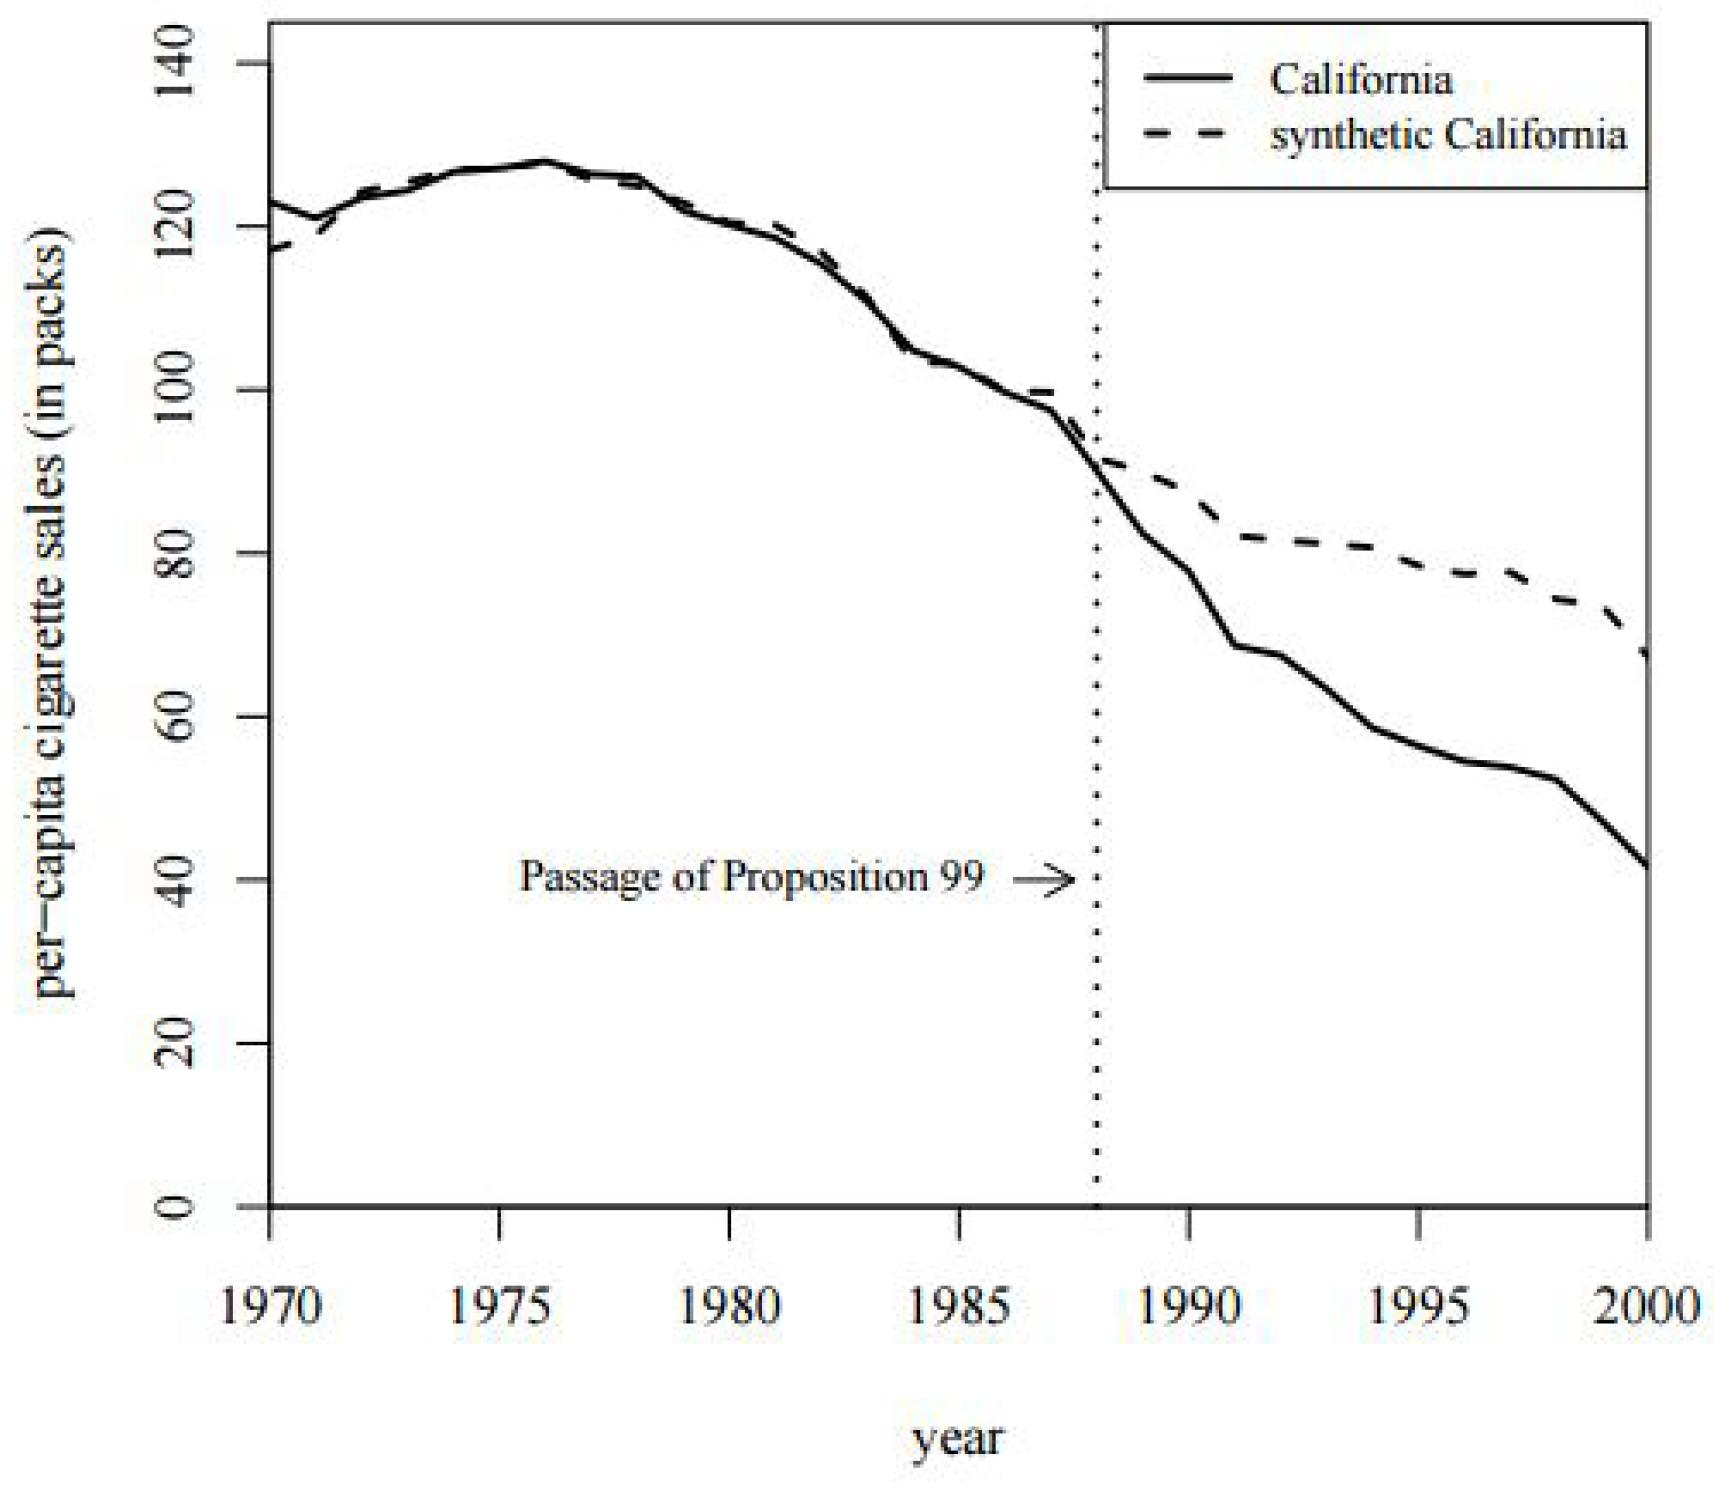
\includegraphics{figure/sc-1.jpg}
\end{figure}
\end{center}
\end{frame}


%\begin{frame}{SC v.s. DID}{Advantages}
%\begin{itemize}
%\item SC builds upon the setting of the standard DID design, but makes the following changes:
%\begin{itemize}
%\vspace{0.2cm}
%%\item[1.] Synthetic Control allows for time-varying individual-specific heterogeneity
%%\vspace{0.2cm}
%
%\item[1] It works in the case where only a single (or small number) of units exposed to the treatment
%\begin{itemize}
%\vspace{0.2cm}
%\item Seek to compensate for the lack of parallel trends 
%by reweighting units to match their pre-exposure trends
%\end{itemize}
%\vspace{0.2cm}
%\item[2] SC takes a serious, data driven approach to forming counterfactuals/selecting the control group
%\vspace{0.2cm}
%\begin{itemize}
%\item  Data-driven procedures reduce discretion in the choice of the control group
%\vspace{0.2cm}
%\end{itemize}
%
%
%\end{itemize}
%\end{itemize}
%\end{frame}
%
%
%
%\begin{frame}{SC v.s. DID}{Disadvantages}
%\begin{itemize}
%\item The benefits of SC method come with three costs:
%\begin{itemize}
%\vspace{0.2cm}
%\item[1.] Large scale (asymptotic) inference cannot be conducted on SC estimators
%\begin{itemize}
%\vspace{0.2cm}
%\item Instead, SC uses \textbf{permutation method} to do statistical inference (compute p-value)
%\vspace{0.2cm}
%\item Recent econometric literature provides new methods for statistical inference
%
%\end{itemize}
%\vspace{0.2cm}
%\item[2.] A key identification assumption is somewhat ambiguous
%\vspace{0.2cm}
%\item[3.] Computational time far exceeds that of DID estimators
%\end{itemize}
%\end{itemize}
%\end{frame}





\begin{frame}{SC v.s. DID}{}
	\begin{itemize}
	
		
		
			\item Treatment Units:
				\vspace{0.2cm}
		\begin{itemize}
			\item DiD: Naturally accommodates multiple treated units
				\vspace{0.2cm}
			\item SCM: Originally designed for a single treated unit 
		\end{itemize}
		
		
		\item Control Group Construction:
						\vspace{0.2cm}
		\begin{itemize}
			\item DID: Uses all untreated units with equal weights and require parallel trends assumption
								\vspace{0.2cm}
			\item SCM: Constructs a synthetic control through data-driven weighted average
		\end{itemize}
		\vspace{0.2cm}
		
		
		
		
		
		
	
	\end{itemize}
\end{frame}



\begin{frame}{SC v.s. DID}{}
	\begin{itemize}
		
		
		
		
		
		\item Data Requirements:
										\vspace{0.2cm}
		\begin{itemize}
			\item DID: Works with limited pre-treatment data (often just one period)
											\vspace{0.2cm}
			\item SCM: Requires extended pre-treatment periods to construct reliable counterfactual
		\end{itemize}
		\vspace{0.2cm}
		
		
		\item Inference Approach:
										\vspace{0.2cm}
		\begin{itemize}
			\item DID: Typically relies on asymptotic statistical inference (t-tests)
												\vspace{0.2cm}
			\item SCM: Uses placebo tests and permutation-based inference
		\end{itemize}
		\vspace{0.2cm}
		
		
		
		
	\end{itemize}
\end{frame}





\title[]  
{Identification}


\author 
{}

%\institute{Institute of Economics, Academia Sinica  \\ Econ, NTU}
%\institute{Institute of Economics, Academia Sinica  \\ IMES/IDAS, NCCU}
\institute{}

%\author 
%{楊子霆 \\ 中研院經濟所}

%\institute 
%{中正大學國際經濟專題研討}




\date
{}


\begin{frame}{}
	\titlepage
\end{frame}




\begin{frame}{Basic Setup: Single Treated Model}{Example}
Alberto Abadie, Alexis Diamond, and Jens Hainmueller (2010), ``\textbf{Synthetic control methods for comparative case studies: Estimating the effect of California's Tobacco Control Program}", Journal of the American Statistical Association	
\begin{itemize}
\vspace{0.2cm}
\item This is one of the first paper using SC method
\vspace{0.2cm}
\begin{itemize}
\item Use this example to go through the key concepts of SC method	
	\vspace{0.2cm}
\item Apply SC method to study the effects of Proposition 99, a large-scale tobacco control program that California implemented in 1988	
\vspace{0.2cm}	
\item A single treated unit with multiple non-treated units		
\end{itemize}	

\end{itemize}
\end{frame}



\begin{frame}{Basic Setup: Single Treated Model}{Example}
\begin{itemize}
\item In 1988, California passed comprehensive tobacco control legislation:
\begin{itemize}
\vspace{0.2cm}
\item Increased cigarette taxes by \$0.25 per pack
\vspace{0.2cm}
\item Funded anti-smoking media campaigns
\vspace{0.2cm}
\item Spurred clean-air ordinances
\end{itemize}
\vspace{0.2cm}
\item They want to estimate the causal effect of the policy on cigarette consumption in California
%\vspace{0.2cm}
%\item Other states that subsequently passed control programs excluded from control group
\end{itemize}
\end{frame}







\begin{frame}{Basic Setup: Single Treated Model}
\begin{itemize}
\item Suppose we observe $J+1$ units over $t=1,...,T$ periods
%with unit $1$ being treated and units $\{2,...,J+1\}$ being unaffected
\vspace{0.2cm}
\item A ``treatment" occurs at period $T_0+1$
\vspace{0.2cm}
\begin{itemize}	
\item Unit $1$ being treated
\vspace{0.2cm}
\item Units $\{2,...,J+1\}$ being unaffected 
\vspace{0.2cm}
\item Pre-treatment period: $1.....T_0$	
\vspace{0.2cm}	
\item Post-treatment period: $T_0+1......T$	
\vspace{0.2cm} 
\end{itemize}
%affects unit $1$ only, and leaves the other $J$ states unaffected 

\item We aim to identify the causal effect of the treatment on unit $1$

\vspace{0.2cm} 
\begin{itemize}
\item Individual treatment effect for unit $1$
\end{itemize}
\end{itemize}

\end{frame}


\begin{frame}{Potential Outcomes Framework}{}
	\begin{itemize}
		
		\item \textcolor{blue}{Treatment}
		\begin{itemize}
			\vspace{0.2cm}
			\item $D_{it}=1$: the units that are treated from periods $T_0+1$ until $T$
			\vspace{0.2cm}
			\item $D_{it}=0$: the units that are always untreated
		\end{itemize}
		
	\end{itemize}
\end{frame}




\begin{frame}{Potential Outcomes Framework}{}
\begin{itemize}
\item \textcolor{blue}{Potential Outcomes}
\vspace{0.2cm}
\begin{itemize}
\item $\mathrm{Y}^{1}_{it}$: the potential outcome we \textit{would} observe for unit $i$ at time $t$ if unit $i$ receives the treatment 
\vspace{0.2cm}
\begin{itemize}
\item Note that the treated unit would receive treatment from periods $T_0+1$ until $T$
\end{itemize}
\vspace{0.2cm}
\item $\mathrm{Y}^{0}_{it}$: the potential outcome we \textit{would} observe for unit $i$ at time $t$ if unit $i$ does not receives the treatment
\end{itemize}
\vspace{0.2cm}
\item Note that \textbf{unit in synthetic control method is usually aggregate level}: country, state, county, or region 



\end{itemize}
\end{frame}









\begin{frame}{Potential Outcomes Framework}{}
\begin{itemize}

\item \textcolor{blue}{Observed Outcomes}
\vspace{0.2cm}
\begin{itemize}
\item $Y_{it}$ is the observed outcome for unit $i$ at time $t$
\vspace{0.2cm}	
\begin{itemize}
\item Observed outcomes before period $T_0+1$:

\begin{equation*}
Y_{it}=\mathrm{Y}^{0}_{it}
\end{equation*}
\item Observed outcomes after period $T_0+1$: 
\begin{equation*}
Y_{it}=\mathrm{Y}^{0}_{it}(1-D_{it})+\mathrm{Y}^{1}_{it}D_{it}
\end{equation*}
%\item Treatment effect for unit $i$ at time $t=1$ is 
%	\begin{equation*}
%	\mathrm{Y}^{1}_{i1}-\mathrm{Y}^{0}_{i1}
%	\end{equation*}
\end{itemize}
\end{itemize}


\end{itemize}
\end{frame}





\begin{frame}{Potential Outcomes Framework}{}
\begin{itemize}
\item Since only unit $1$ is treated, we aim to estimate the causal effect of treatment over time ($T_{0}+1,.....,T$) for the treated unit $1$
\begin{equation*}
\alpha_{1t}=(\alpha_{1T_{0}+1},...,\alpha_{1T})
\end{equation*}
where for $t>T_0$:
\begin{equation*}
\alpha_{1t}=\underbrace{Y^1_{1t}}_{\text{observed}}-\underbrace{Y^0_{1t}}_{\text{counterfactual}}
\end{equation*}
\vspace{0.2cm}
\item We need to construct the \textbf{unobserved counterfactual} for unit $1$
\end{itemize}
\end{frame}









\title[]  
{Estimation}


\author 
{}

%\institute{Institute of Economics, Academia Sinica  \\ Econ, NTU}
%\institute{Institute of Economics, Academia Sinica  \\ IMES/IDAS, NCCU}
\institute{}

%\author 
%{楊子霆 \\ 中研院經濟所}

%\institute 
%{中正大學國際經濟專題研討}




\date
{}


\begin{frame}{}
\titlepage
\end{frame}




\begin{frame}{SC Estimation}




\begin{equation*}
\alpha_{1t}=\underbrace{Y^1_{1t}}_{\text{observed}}-\underbrace{Y^0_{1t}}_{\text{counterfactual}}
\end{equation*}	
\begin{itemize}
\item SC method suggests treatment effect can be estimated by the simple difference:

\begin{equation*}
\hat{\alpha}_{1t}=Y_{1t}-\sum^{J+1}_{i=2}w^*_{i}Y_{it}
\end{equation*}
	

\end{itemize}
\end{frame}






\begin{frame}{SC Estimation}
\begin{itemize}
	\item Choose weights $W=(w^{*}_{2},...,w^{*}_{J+1})$$\in$ [0,1] to minimize difference in pre-treatment characteristics $X$ between treated and weighted average of non-treated units
	\vspace{0.2cm}
	\begin{equation*}
		\begin{aligned}
			W^* = \argmin\limits_{W} & \sum_{k=1}^{K} v_k\left(X_{1k} - \sum_{i=2}^{J+1} w_i X_{ik}\right)^2 \\
			\text{subject to } & \sum_{i=2}^{J+1} w_i = 1 
		\end{aligned}
	\end{equation*}

\begin{itemize}
	\item $X_{1k}$ is the $k$-th predictor variable for the treated unit
				\vspace{0.2cm}
		\item $X_{jk}$ is the $k$-th predictor variable for non-treated unit $j$
					\vspace{0.2cm}
			\item $v_k$ represents relative importance of each predictor variable (chosen by cross-validation)
\end{itemize}
\end{itemize}
\end{frame}





\begin{frame}{SC Estimation}
	\begin{itemize}
		
	\item Predictor variables $X$ typically include:
				\vspace{0.2cm}
			\begin{itemize}
					\item Pre-treatment outcomes $Y_{1},...,Y_{T_0}$ (most predictive)
								\vspace{0.2cm}
					\item Other observed covariates $Z$ 
				\end{itemize}
			\vspace{0.2cm}
			\item Different predictor variables $X$ and choice of weights $v_k$ result in distinct synthetic units
	\end{itemize}
\end{frame}





%\begin{frame}{Synthetic Control Method (SCM) Estimation - I}
%	\begin{itemize}
%		\item Create a "synthetic control unit" by weighted averaging of non-treated units to match pre-treatment characteristics of the treated unit
%		\vspace{0.2cm}
%		\item Choose weights $W=(w_{2},...,w_{J+1})$ $\in$ [0,1] to minimize difference in pre-treatment characteristics $X$ between treated and weighted average of non-treated units:
%		\vspace{0.2cm}
%		\begin{equation*}
%			\begin{aligned}
%				W^* = \argmin\limits_{W} & \sum_{k=1}^{K} v_k\left(X_{1k} - \sum_{j=2}^{J+1} w_j X_{jk}\right)^2 \\
%				\text{subject to } & \sum_{j=2}^{J+1} w_j = 1, \; w_j \geq 0 \; \forall j \in \{2,...,J+1\}
%			\end{aligned}
%		\end{equation*}
%		\item Where:
%		\begin{itemize}
%			\item $X_{1k}$ is the $k$-th predictor variable for the treated unit
%			\item $X_{jk}$ is the $k$-th predictor variable for non-treated unit $j$
%			\item $v_k$ represents relative importance of each predictor variable (typically chosen by cross-validation)
%		\end{itemize}
%	\end{itemize}
%\end{frame}
%
%\begin{frame}{Synthetic Control Method (SCM) Estimation - II}
%	\begin{itemize}
%		\item Predictor variables $X$ typically include:
%		\begin{itemize}
%			\item Pre-treatment outcomes $Y_{1},...,Y_{T_0}$ (most predictive)
%			\item Other observed covariates $Z$ (demographics, economic indicators, etc.)
%		\end{itemize}
%		\vspace{0.3cm}
%		\item Different predictor variables $X$ and choice of weights $v_k$ result in distinct synthetic units
%		\vspace{0.3cm}
%		\item Treatment effect estimation:
%		\begin{equation*}
%			\hat{\tau}_{1t} = Y_{1t} - \sum_{j=2}^{J+1} w^*_j Y_{jt}, \quad \forall t > T_0
%		\end{equation*}
%		\vspace{0.2cm}
%		\item Method advantages:
%		\begin{itemize}
%			\item No need for random assignment of treatment
%			\item Allows for time-varying treatment effects
%			\item Transparent weight selection process
%			\item Avoids extrapolation issues
%		\end{itemize}
%	\end{itemize}
%\end{frame}




\begin{frame}{Assumptions of SC}
	\begin{itemize}
		\item Assume potential outcome if unit $1$ would not receive treatment $Y^0_{1t}$ can be expressed as follows:
		\begin{equation*}
			Y^0_{1t}=\delta_t+\theta_tZ_1+\lambda_t\mu_1+\varepsilon_{1t}
		\end{equation*}
		\begin{itemize}
			\item $\delta_t$ are common time effects (e.g. year fixed effects)
			\vspace{0.2cm}
			\item $Z_1$ are the observed, pre-treatment covariates
			\vspace{0.2cm}
			\item $\mu_1$ are \textbf{permanent} unobserved variables
			\vspace{0.2cm}
			\item $\varepsilon_{1t}$ are unobserved transitory shocks at the unit level with zero mean
			\vspace{0.2cm}
		\end{itemize}
		\item This assumption allows time-varying responsses of multiple unobserved factors ($\lambda_t\mu_1$) 
		
		%heterogenous responsses to multiple unobserved factors ($\lambda_t\mu_i$) 
		%and embeds time-trend models
		\vspace{0.2cm}
		\item However, it implicitly assumes \textbf{the number of unobservable factors $\mu_1$ are fixed over the period} 
		\vspace{0.2cm}
		\begin{itemize}
			\item No structural breaks
		\end{itemize}
		
		
	\end{itemize}
\end{frame}



%\begin{frame}{Why SCM Relaxes the Parallel Trends Assumption}
%	\begin{itemize}
%		\item Recall the factor model: $Y^0_{1t}=\delta_t+\theta_tZ_1+\lambda_t\mu_1+\varepsilon_{1t}$
%		\vspace{0.2cm}
%		
%		\item SCM creates a synthetic control by selecting weights $W^*$ such that:
%		\begin{equation*}
%			\sum_{j=2}^{J+1} w^*_j Y_{jt} \approx Y_{1t} \text{ for } t < T_0
%		\end{equation*}
%		
%		\item This implicitly ensures:
%		\begin{equation*}
%			\sum_{j=2}^{J+1} w^*_j \mu_j \approx \mu_1 \text{ and } \sum_{j=2}^{J+1} w^*_j Z_j \approx Z_1
%		\end{equation*}
%		
%		\vspace{0.2cm}
%		
%		\item Three key advantages over DiD:
%		\begin{itemize}
%			\item \textbf{Non-parallel pre-treatment trends}: By matching the entire pre-treatment trajectory, SCM captures unit-specific trends rather than assuming parallel paths
%			\vspace{0.2cm}
%			
%			\item \textbf{Time-varying effects of unobserved variables}: The term $\lambda_t\mu_1$ allows unobserved factors to have different effects at different time points
%			\vspace{0.2cm}
%			
%			\item \textbf{Heterogeneous responses to common shocks}: Units with different characteristics ($\mu_j$) can respond differently to common time effects, and SCM accounts for this by matching these characteristics
%		\end{itemize}
%		
%		\vspace{0.2cm}
%		
%		\item Example: During economic recessions ($\delta_t$), regions with different industrial compositions ($\mu_j$) may experience different impacts—SCM can capture this heterogeneity
%	\end{itemize}
%\end{frame}




\begin{frame}{SC Estimation}
\begin{itemize}

\item Ideally, one would want to select $W^{*}$ such that

\begin{equation*}
\sum^{J+1}_{j=2}w^*_{i}Z_{i} = Z_{1}  
\end{equation*}

\begin{equation*}
\sum^{J+1}_{j=2}w^*_{i}\mu_{i} = \mu_{1}  
\end{equation*}

\item Thus, causal effect of treatment $\hat{\alpha}_{1t}$ is unbiased 	

\end{itemize}
\end{frame}







\begin{frame}{SC Estimation}
\begin{itemize}
	
	\item Problem: \textbf{$\mu_{i}$ is unobserved}
\end{itemize}
\end{frame}





\begin{frame}{SC Estimation}
\begin{itemize}

\item Solution: Choose $W=(w^{*}_{1},...,w^{*}_{J})$ satisfying

\begin{equation*}
\begin{aligned}
&\sum^{J+1}_{i=2}w^*_{i}Z_{i} = Z_{1}, \\ 
&\sum^{J+1}_{i=2}w^*_{i}Y_{i1} = Y_{11},  \\
&\sum^{J+1}_{i=2}w^*_{i}Y_{i2} = Y_{12},...,  \\
&\sum^{J+1}_{i=2}w^*_{i}Y_{iT_{0}} = Y_{1T_{0}}    
\end{aligned}
\end{equation*}

\end{itemize}
\end{frame}






\begin{frame}{SC Estimation}
\begin{itemize}
\item \textbf{SC Theorem}: Suppose there exists $W^*$ such that the SC matches the treated unit in the pre-treatment period ($\forall t\in\{1,...,T_0\}$): 
\begin{align*}
\sum^{J+1}_{i=2}w^*_{i}Y_{it}&=Y_{1t} \\
\sum^{J+1}_{i=2}w^*_{i}Z_i&=Z_1,
\end{align*}
and $\sum^{T_0}_{t=1}\lambda'_t\lambda_t$ is non-singluar. Then for all $t>T_0$ we have
\begin{equation*}
\mathbb{E}\left[Y^0_{1t}-\sum^{J+1}_{i=2}w^*_{i}Y_{it}\right]\rightarrow 0
\end{equation*}
as $T_0\rightarrow\infty$ 

%or if $T_0$ is large relative to $\varepsilon_{i,t}$
\end{itemize}
\end{frame}


%
%\begin{frame}{SC: Model Setup}
%	\begin{itemize}
%		\item \textbf{Data Generating Process}:
%		\begin{equation*}
%			Y_{it} = \delta_t + \theta_t Z_i + \lambda_t \mu_i + \epsilon_{it}
%		\end{equation*}
%		where
%		\begin{itemize}
%			\item $\delta_t$: time fixed effects (e.g., general economic conditions)
%			\item $\theta_t Z_i$: observed characteristics with time-varying coefficients
%			\item $\lambda_t \mu_i$: unobserved common factors ($\lambda_t$) with unit-specific loadings ($\mu_i$)
%			\item $\epsilon_{it}$: transitory shocks
%		\end{itemize}
%	\end{itemize}
%\end{frame}
%\begin{frame}{SC: Identification}
%	\begin{itemize}
%		\item If there exists weights $W^$ such that:
%		\begin{align}
%			\sum_{j=2}^{J+1} w_j^* Z_j &= Z_1 \text{ (matching on observables)}\
%			\sum_{j=2}^{J+1} w_j^* \mu_j &= \mu_1 \text{ (matching on factor loadings)}
%		\end{align}
%		\item Then the synthetic control will approximate the counterfactual:
%		\begin{equation*}
%			Y_{1t}^0 \approx \sum_{j=2}^{J+1} w_j^* Y_{jt}
%		\end{equation*}
%		\item The condition $\sum_{t=1}^{T_0} \lambda_t'\lambda_t$ non-singular ensures:
%		\begin{itemize}
%			\item Common factors are linearly independent
%			\item Sufficient variation to identify factor loadings
%			\item Pre-treatment fit implies matching on factor loadings
%		\end{itemize}
%	\end{itemize}
%\end{frame}
%
%
%\begin{frame}{SC: Implementation}
%	\begin{itemize}
%		\item In practice, we:
%		\begin{equation*}
%			\begin{aligned}
%				W^* = \argmin\limits_{W} & \sum_{k=1}^{K} v_k\left(X_{1k} - \sum_{j=2}^{J+1} w_j X_{jk}\right)^2 \
%				\text{subject to } & \sum_{j=2}^{J+1} w_j = 1, \quad w_j \geq 0
%			\end{aligned}
%		\end{equation*}
%		\item Where $X$ includes both $Z$ and pre-treatment $Y$
%		\item Good pre-treatment fit suggests we've matched on both:
%		\begin{itemize}
%			\item Observable characteristics ($Z$)
%			\item Unobservable factor loadings ($\mu$)
%		\end{itemize}
%	\end{itemize}
%\end{frame}





\begin{frame}{SC Estimation}{Graphical Representation}
\begin{center}
	\begin{figure}[p]
		\centering
		%\scalebox{0.98}{\includegraphics{did_1.jpg}}
		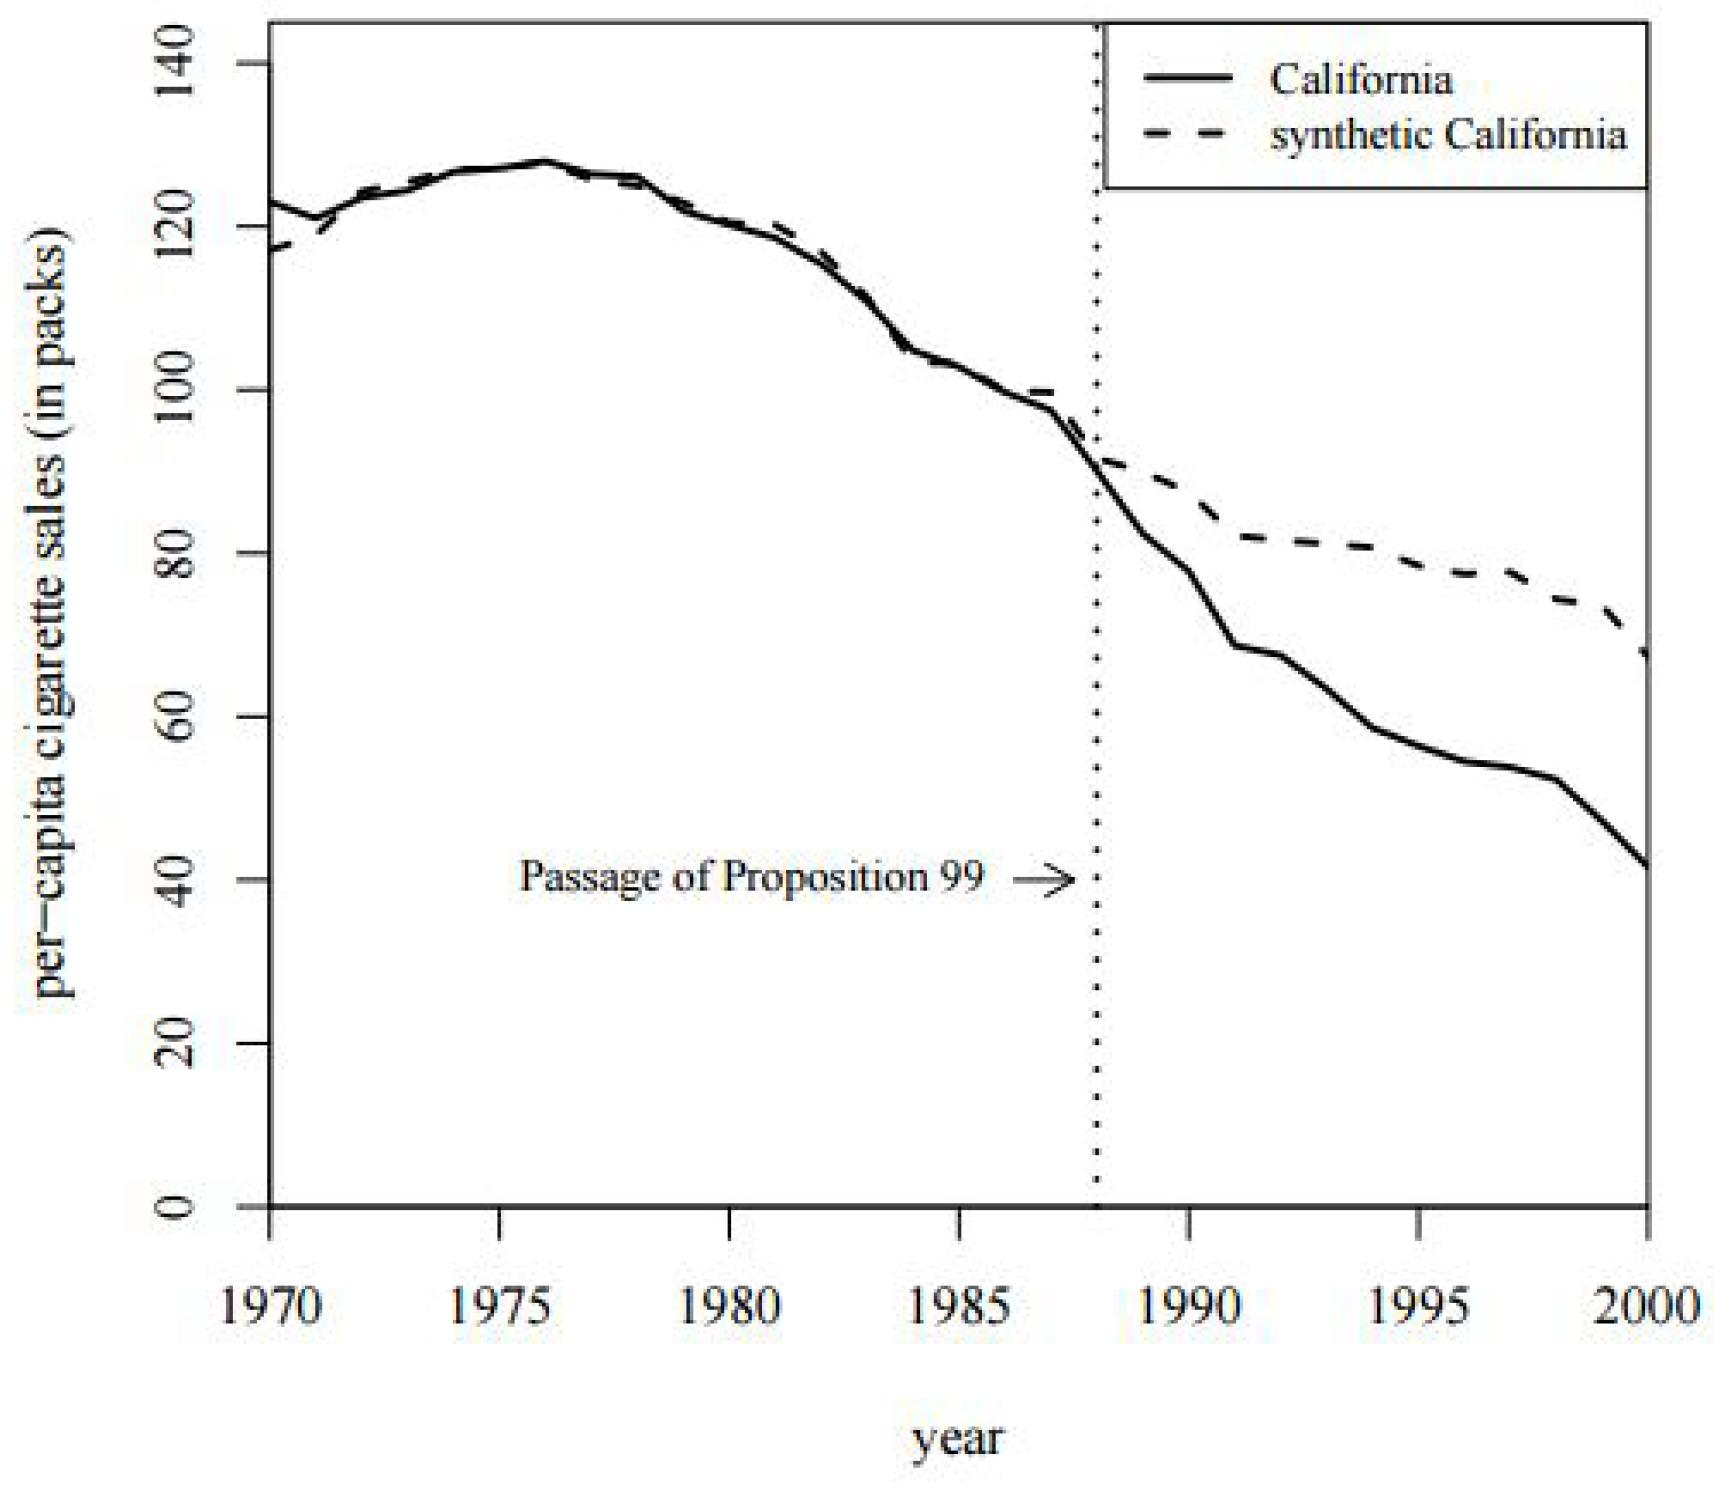
\includegraphics{figure/sc-1.jpg}
	\end{figure}
\end{center}
\end{frame}



\begin{frame}{SC Estimation}{Intuition}
\begin{itemize}
%\item If the conditions are met, the the ``synthetic control" associated with $W^*$ replicates the missing counterfactual
%\vspace{0.2cm}
\item An approximately unbiased estimator of causal effect of treatment $\alpha_{1t}$ is then given by:
\begin{equation*}
\hat{\alpha}_{1t}=Y_{1t}-\sum^{J+1}_{i=2}w^*_iY_{it}
\end{equation*}

\begin{itemize}
\item The difference between the observed outcome and the outcome of synthetic unit.

\end{itemize}

\vspace{0.2cm}
\item Beauty of SC is that even though the \textbf{$\mu_1$ are unobservable}, fitting $\{Y_{1t},Z_{1}\}$ is sufficient to match the process
\vspace{0.2cm}
\item \textbf{Intuition:} a synthetic cohort can fit ($Z_{1},Y_{11},...Y_{1T_{0}} $) for a large $T_{0}$ only if it fits ($Z_{1},\mu_{1} $)
\end{itemize}
\end{frame}


%\begin{frame}{Why SCM Relaxes the Parallel Trends Assumption}
%	\begin{itemize}
%	
%			\item DID design requires that the difference between treated and untreated units remains constant over time in the absence of treatment (Parallel Trends Assumption)
%			
%			
%			
%			\item By matching the entire pre-treatment trajectory, SC captures unit-specific trends rather than assuming parallel trend
%			
%
%			
%			
%		
%			
%		
%	\end{itemize}
%\end{frame}



%\begin{frame}{Why SCM Relaxes the Parallel Trends Assumption}
%	\begin{itemize}
%		\item \textbf{DiD Assumption}: In the absence of treatment, the difference between treated and control units would remain constant over time (Parallel Trends)
%		\vspace{0.3cm}
%		
%		\item \textbf{DiD Factor Model}: $Y^0_{it} = \alpha_i + \delta_t + \varepsilon_{it}$
%		\begin{itemize}
%			\item Time-invariant unit effects ($\alpha_i$) + common time effects ($\delta_t$)
%		\end{itemize}
%		\vspace{0.3cm}
%		
%		\item \textbf{SCM Approach}: Instead of assuming parallel trends, SCM creates a counterfactual by:
%		\begin{itemize}
%			\item Matching the entire pre-treatment trajectory of the treated unit
%			\item Allowing for time-varying effects of unobserved factors ($\lambda_t\mu_i$)
%			\item Directly constructing the control unit as a weighted average of donor units
%		\end{itemize}
%		\vspace{0.3cm}
%		
%		\item \textbf{Implication}: SCM can accommodate non-parallel trends and heterogeneous responses to common shocks across units
%	\end{itemize}
%\end{frame}



\begin{frame}{Example: Abadie et. al (2010)}{Results: Unit Weights for SC}
\begin{center}
	\begin{figure}[p]
		\centering
		\scalebox{0.65}{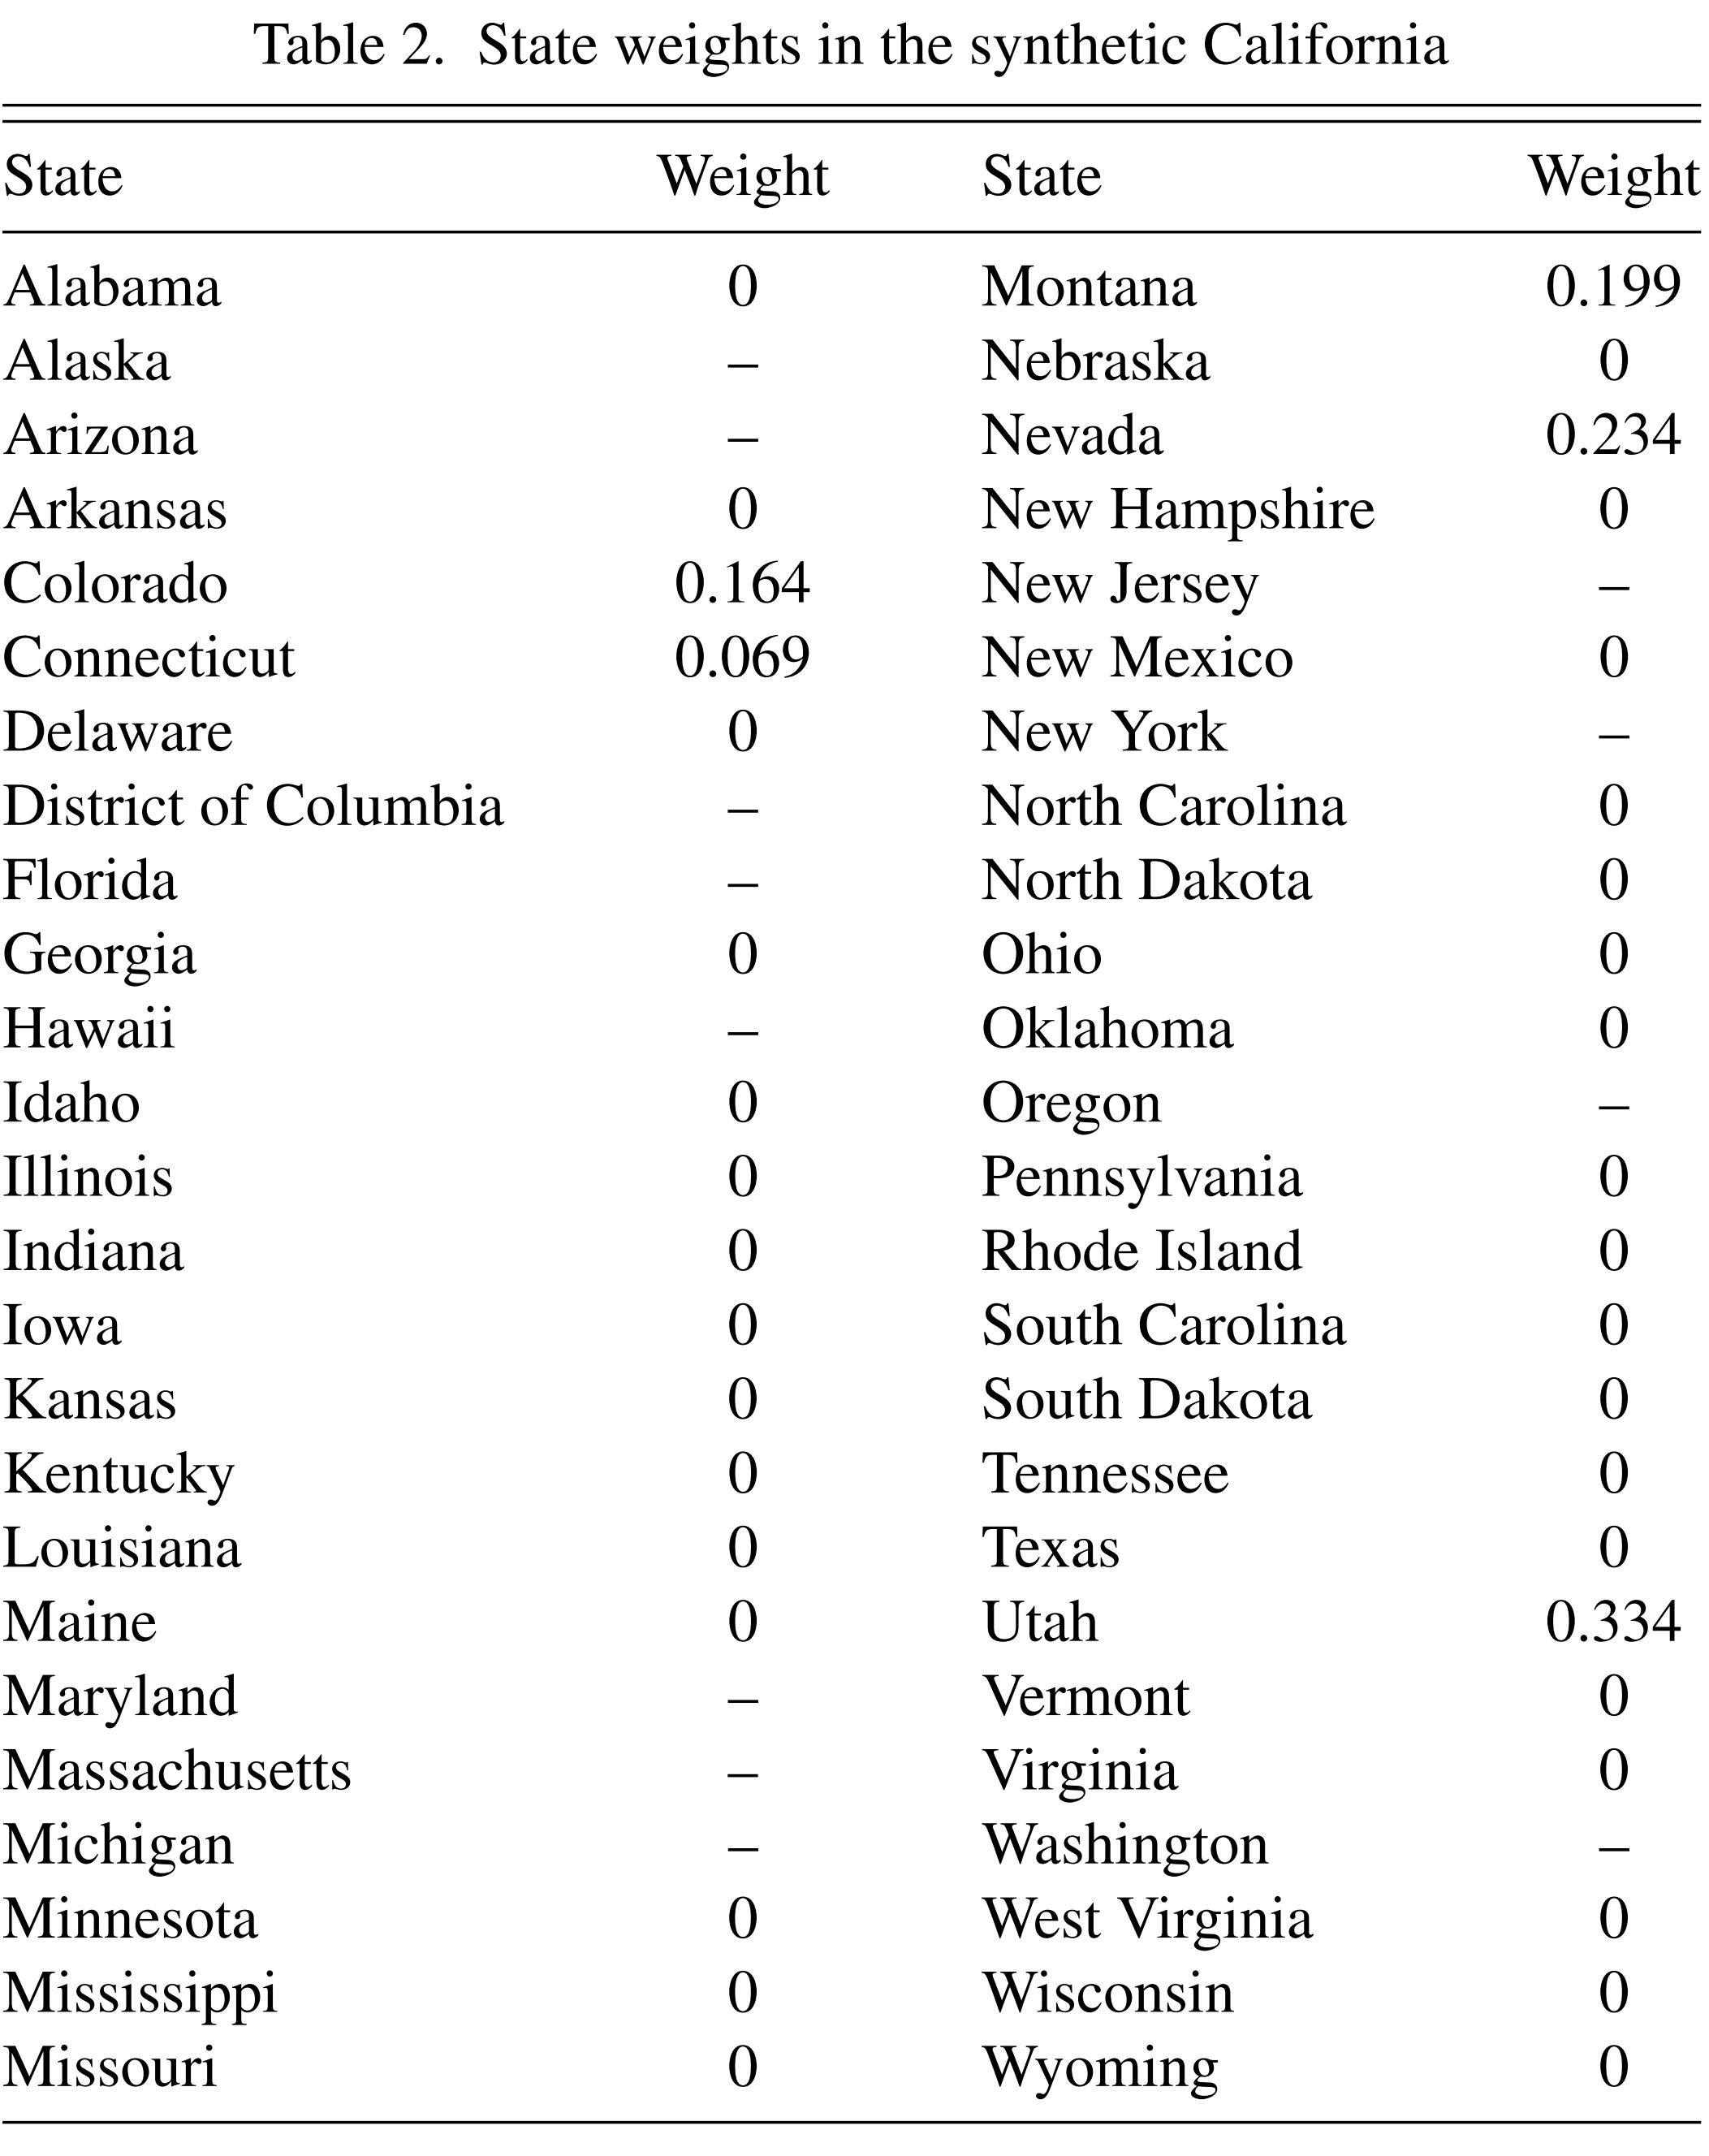
\includegraphics{figure/sc_t2.jpg}}
		%\includegraphics{sc-5.jpg}
	\end{figure}
\end{center}
\end{frame}


\begin{frame}{Example: Abadie et. al (2010)}{Comparison of Synthetic Fit and Simple Average}
\begin{table}[p]
\centering
%\extrarowheight = 3pt 
\scalebox{0.95}{
\begin{tabular}{lccc}
\hline
& \multicolumn{2}{c}{California}    & Average of  \\
Variables & Real        & Synthetic           & 38 control states \\
\hline
Ln (GDP per capita)         & 10.08 & 9.86  & 9.86   \\
Percent aged 15-24          & 17.40 & 17.40 & 17.29  \\
Retail price                & 89.42 & 89.41 & 87.27  \\
Beer consumption per capita & 24.28 & 24.20 & 23.75  \\
Cigarette sales per capita 1988 & 90.10  & 91.62  & 114.20  \\
Cigarette sales per capita 1980 & 120.20 & 120.43 & 136.58  \\
Cigarette sales per capita 1975 & 127.10 & 126.99 & 132.81  \\
\hline
\end{tabular}}
\end{table}
\end{frame}





\title[]  
{Statistical Inference}


\author 
{}

%\institute{Institute of Economics, Academia Sinica  \\ Econ, NTU}
%\institute{Institute of Economics, Academia Sinica  \\ IMES/IDAS, NCCU}
\institute{}

%\author 
%{楊子霆 \\ 中研院經濟所}

%\institute 
%{中正大學國際經濟專題研討}




\date
{}


\begin{frame}{}
	\titlepage
\end{frame}




\begin{frame}{Statistical Inference of SC}
\begin{itemize}
\item Large-sample asymptotic inference is not possible with SC
\vspace{0.2cm}
\item Abadie et. al (2010) suggest the use of \textbf{permutation methods} for inference 
\vspace{0.2cm}
	\begin{itemize}
	%\item Similar to Fisher's exact test
	\item Does not rely on large-sample asymptotics
	%	\item Provides exact inference under exchangeability
\end{itemize}
\vspace{0.2cm}
\item \textbf{Main Idea:} 
\vspace{0.2cm}
\begin{itemize}
\item How often would we obtain results of this magnitude if we had chosen a state at random for the study instead of California ?
\vspace{0.2cm}

\item Run placebo studies by applying the SC method to states that did NOT receive treatment
\vspace{0.2cm}
\begin{itemize}
\item  If the placebo studies create gaps of magnitude similar to the one estimated for California 
\vspace{0.2cm}
\item Then our interpretation is that
our analysis does NOT provide significant evidence of causal effect
\end{itemize}
\end{itemize}
\end{itemize}
\end{frame}










\begin{frame}{Permutation Test: Basic Steps}
	\begin{itemize}
		\item \textbf{Step 1:} Estimate treatment effect for treated unit (e.g., California)
		\begin{equation*}
			\hat{\alpha}_{1t} = Y_{1t} - \sum_{j=2}^{J+1} w_i^* Y_{it}, \quad t > T_0
		\end{equation*}
		\vspace{0.2cm}
		\item \textbf{Step 2:} Conduct placebo studies
				\vspace{0.2cm}
		\begin{itemize}
			\item Apply SC to each control unit in donor pool as if it were treated
					\vspace{0.2cm}
			\item Calculate placebo effects $\{\hat{\alpha}_{2t},...,\hat{\alpha}_{J+1,t}\}$
		%			\vspace{0.2cm}
		%	\item Compare magnitude of effects across units
		\end{itemize}
		\vspace{0.2cm}
		\item \textbf{Key Question:} How unusual is the estimated effect for California compared to effects we estimate for units that did NOT receive treatment?
	\end{itemize}
\end{frame}

\begin{frame}{Permutation Test: Statistical Inference}
	\begin{itemize}
		\item \textbf{Step 3:} Calculate empirical p-value
		\begin{itemize}
			\item Plot all estimated effect (treated and placebos) for visual inspection
			\vspace{0.2cm}
			\item Calculate empirical p-value at each post-treatment time $t$:
			\begin{equation*}
				p_{1t}=\dfrac{\sum^{J+1}_{i=2}\mathbf{1}\{\hat{\alpha}_{it}\geq\hat{\alpha}_{1t}\}}{J}
			\end{equation*}
			where $\mathbf{1}\{\cdot\}$ is the indicator function
		\end{itemize}
		\vspace{0.2cm}
		\item \textbf{Interpretation:} 
		\begin{itemize}
			\item Small $p_{1t}$: treatment effect is unusually large compared to placebo effects
					\vspace{0.2cm}
			\item Large $p_{1t}$: cannot distinguish treatment effect from random chance
		\end{itemize}
	\end{itemize}
\end{frame}


\begin{frame}{SC Analysis for Treated State}{California}
	\begin{center}
		\begin{figure}[p]
			\centering
			%\scalebox{0.98}{\includegraphics{did_1.jpg}}
			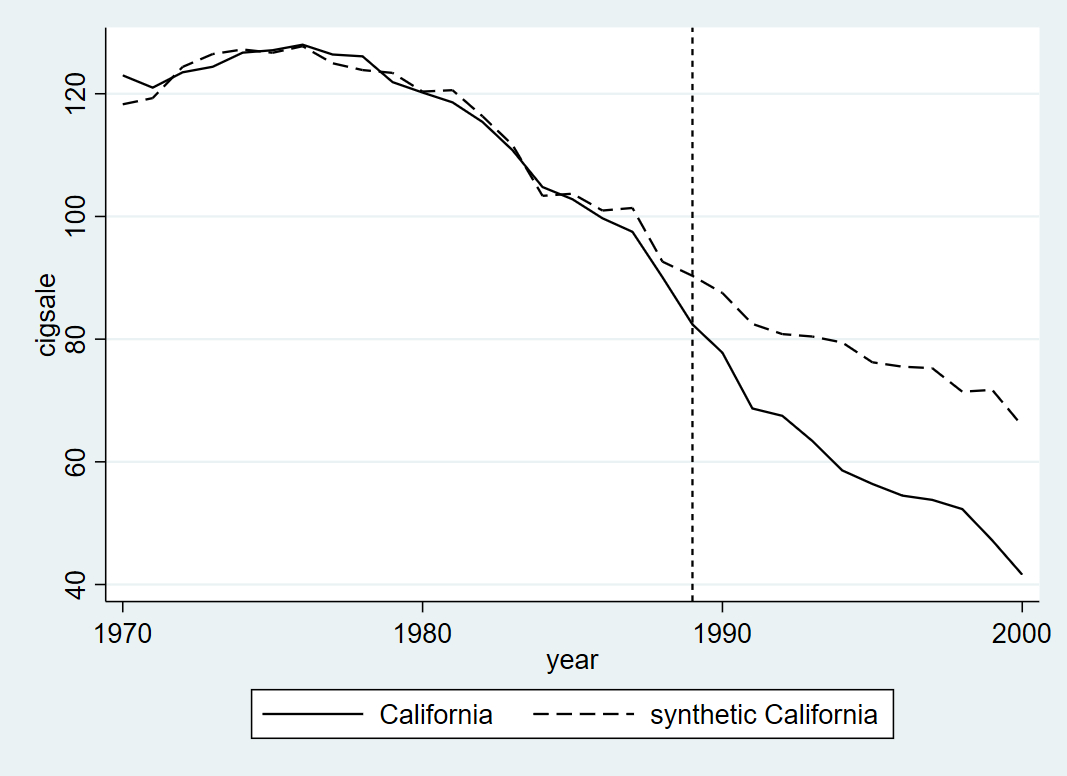
\includegraphics[width=0.9\textwidth]{figure/CA.png}
		\end{figure}
	\end{center}
\end{frame}



\begin{frame}{SC Analysis for Non-treated States}{Alabama}
	\begin{center}
		\begin{figure}[p]
			\centering
			%\scalebox{0.98}{\includegraphics{did_1.jpg}}
			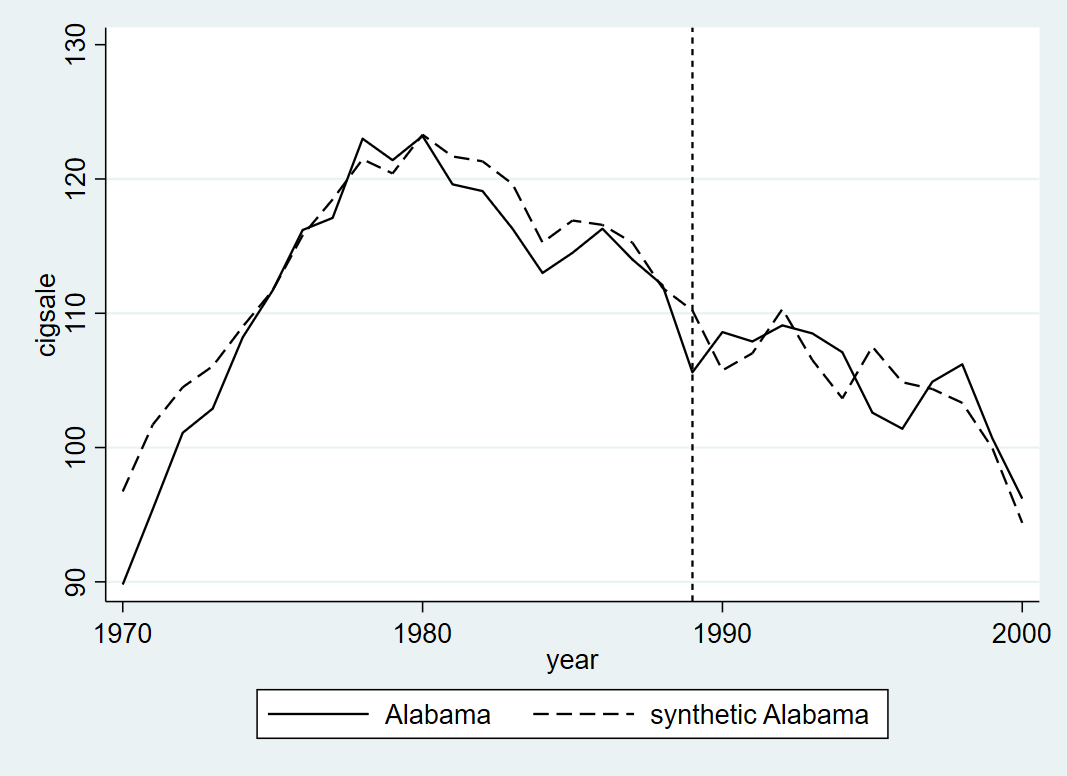
\includegraphics[width=0.9\textwidth]{figure/state1.png}
		\end{figure}
	\end{center}
\end{frame}


\begin{frame}{SC Analysis for Non-treated States}{Arkansas}
	\begin{center}
		\begin{figure}[p]
			\centering
			%\scalebox{0.98}{\includegraphics{did_1.jpg}}
			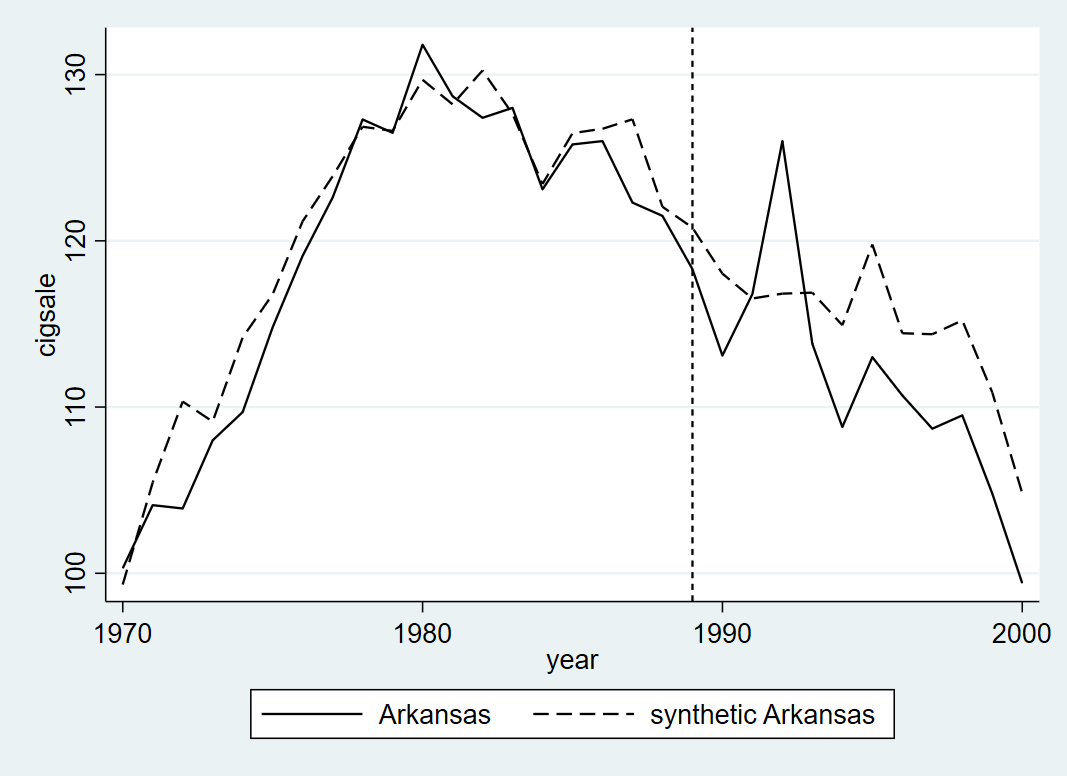
\includegraphics[width=0.9\textwidth]{figure/state2.png}
		\end{figure}
	\end{center}
\end{frame}


\begin{frame}{SC Analysis for Non-treated States}{Colorado}
	\begin{center}
		\begin{figure}[p]
			\centering
			%\scalebox{0.98}{\includegraphics{did_1.jpg}}
		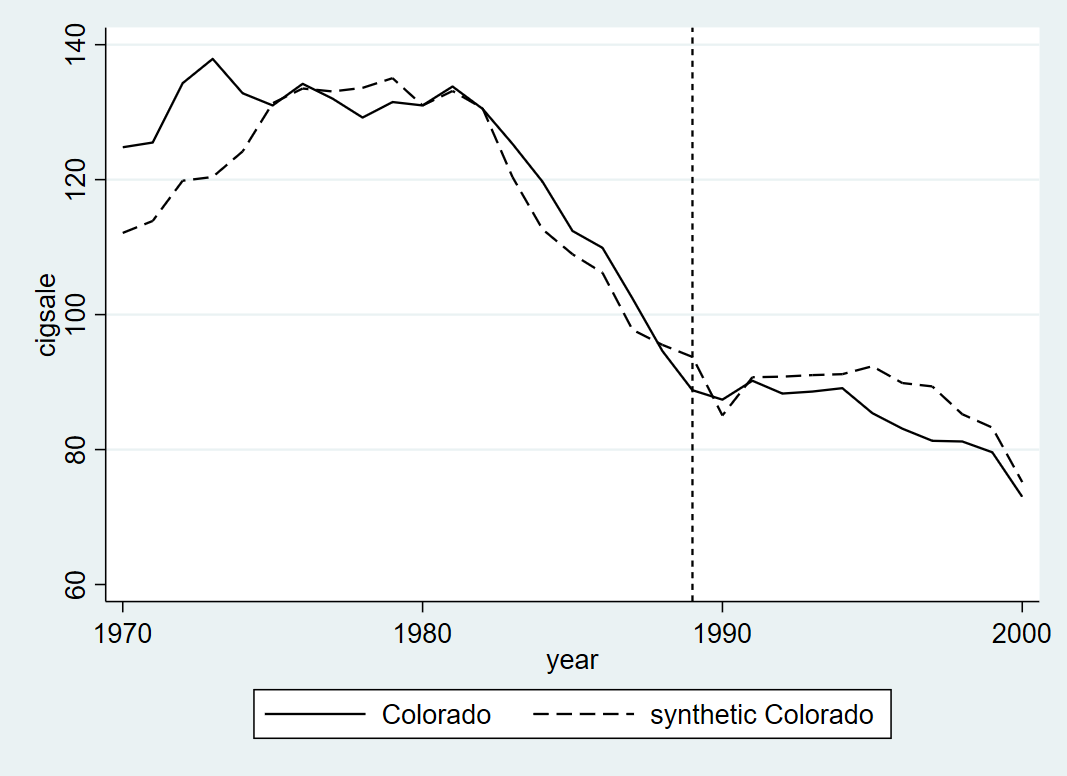
\includegraphics[width=0.9\textwidth]{figure/state4.png}
		\end{figure}
	\end{center}
\end{frame}


\begin{frame}{SC Analysis for Non-treated States}{Connecticut}
	\begin{center}
		\begin{figure}[p]
			\centering
			%\scalebox{0.98}{\includegraphics{did_1.jpg}}
			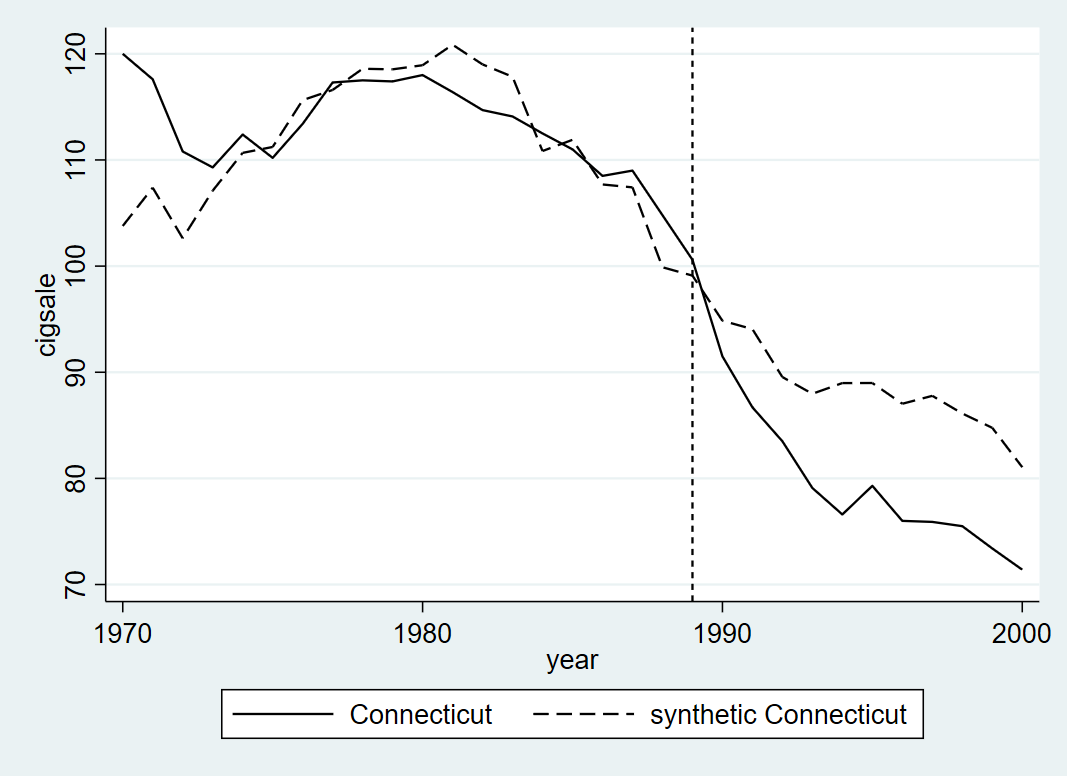
\includegraphics[width=0.9\textwidth]{figure/state5.png}
		\end{figure}
	\end{center}
\end{frame}


\begin{frame}{SC Estimates for California vs. Non-treated States}{Use All Placebo Estimates}
\begin{center}
\begin{figure}[p]
\centering
%\scalebox{0.98}{\includegraphics{did_1.jpg}}
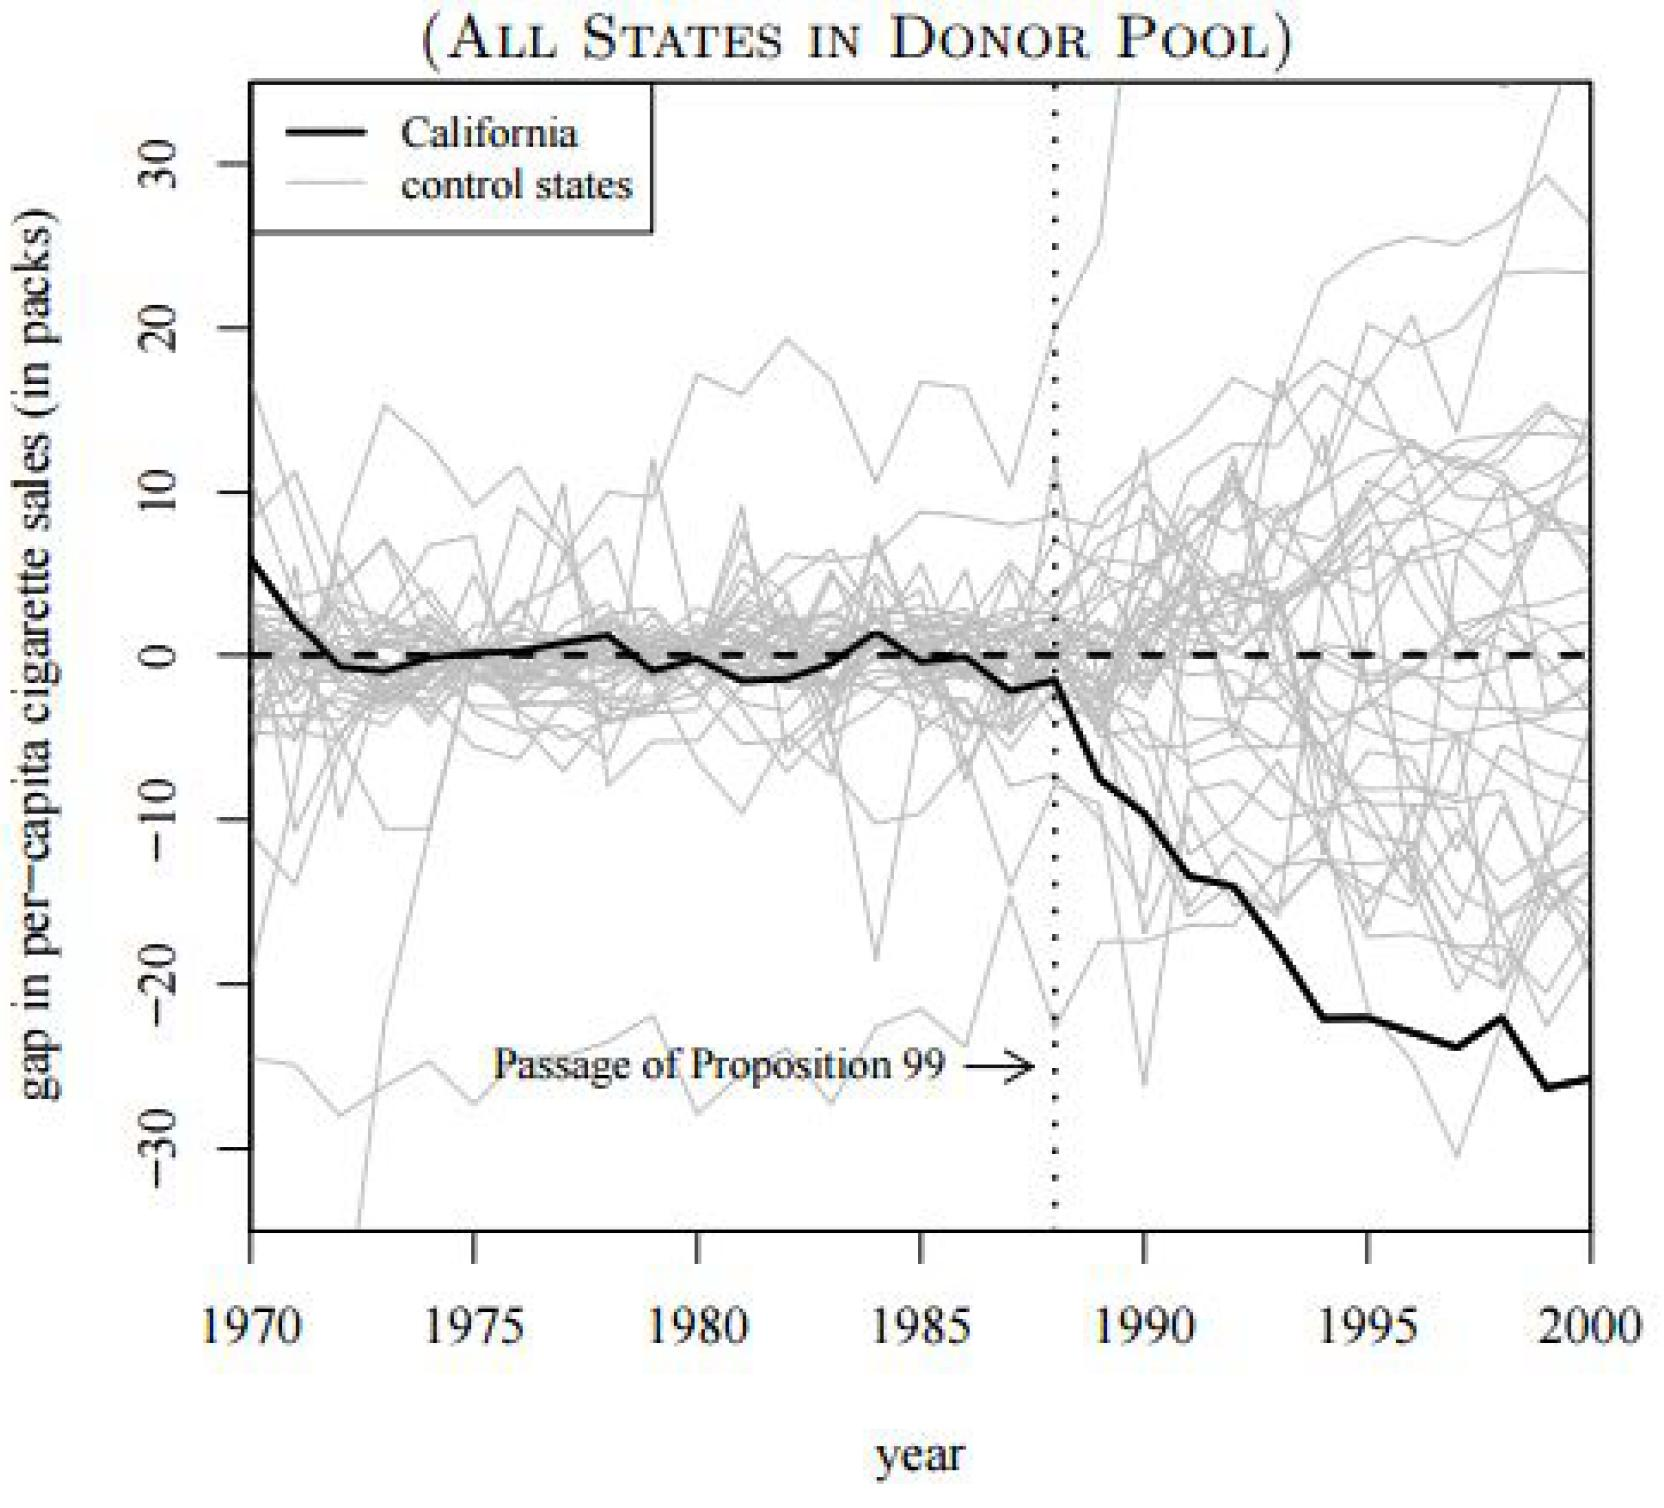
\includegraphics{figure/sc-4.jpg}
\end{figure}
\end{center}
\end{frame}



\begin{frame}{Statistical Inference of SC}
\begin{itemize}
\item The placebo effects may be quite large if those units where NOT matched well in the pre-treatment period
\vspace{0.2cm}
\item For example, when the SC fit is bad, we may get erroneous inferences 
\vspace{0.2cm}
\begin{itemize}
\item Look at bottom gray line in the above figure
\vspace{0.2cm}
\end{itemize}
\item This would cause too large p-values 


\end{itemize}
\end{frame}


\begin{frame}{Statistical Inference of SC}{}
	\begin{itemize}
		\item To control for this, one may want to \textbf{adjust $\hat{\alpha}_{it}$ for the quality of the pre-treatment matches}
		\vspace{0.2cm}
		
		
		\item \textbf{Method 1:}
				\vspace{0.2cm}
			\begin{itemize}
		\item Removing observations with too big Root Mean Squared Predictive Error (RMSPE) during the pre-treatment period
		
		
		\begin{equation*}
			RMSPE^{pre}_{i}= 	\sqrt{\dfrac{			\sum^{T_{0}}_{t=1}(Y_{it} - Y^{SC}_{it})^{2}}{T_{0}}}
			
		

		\end{equation*}
		
			\end{itemize}
	\end{itemize}
\end{frame}







\begin{frame}{SC Estimates for CA vs. Placebo Treatments}{Use High-Quality Placebo Estimates}
\begin{center}
	\begin{figure}[p]
		\centering
		\scalebox{0.85}{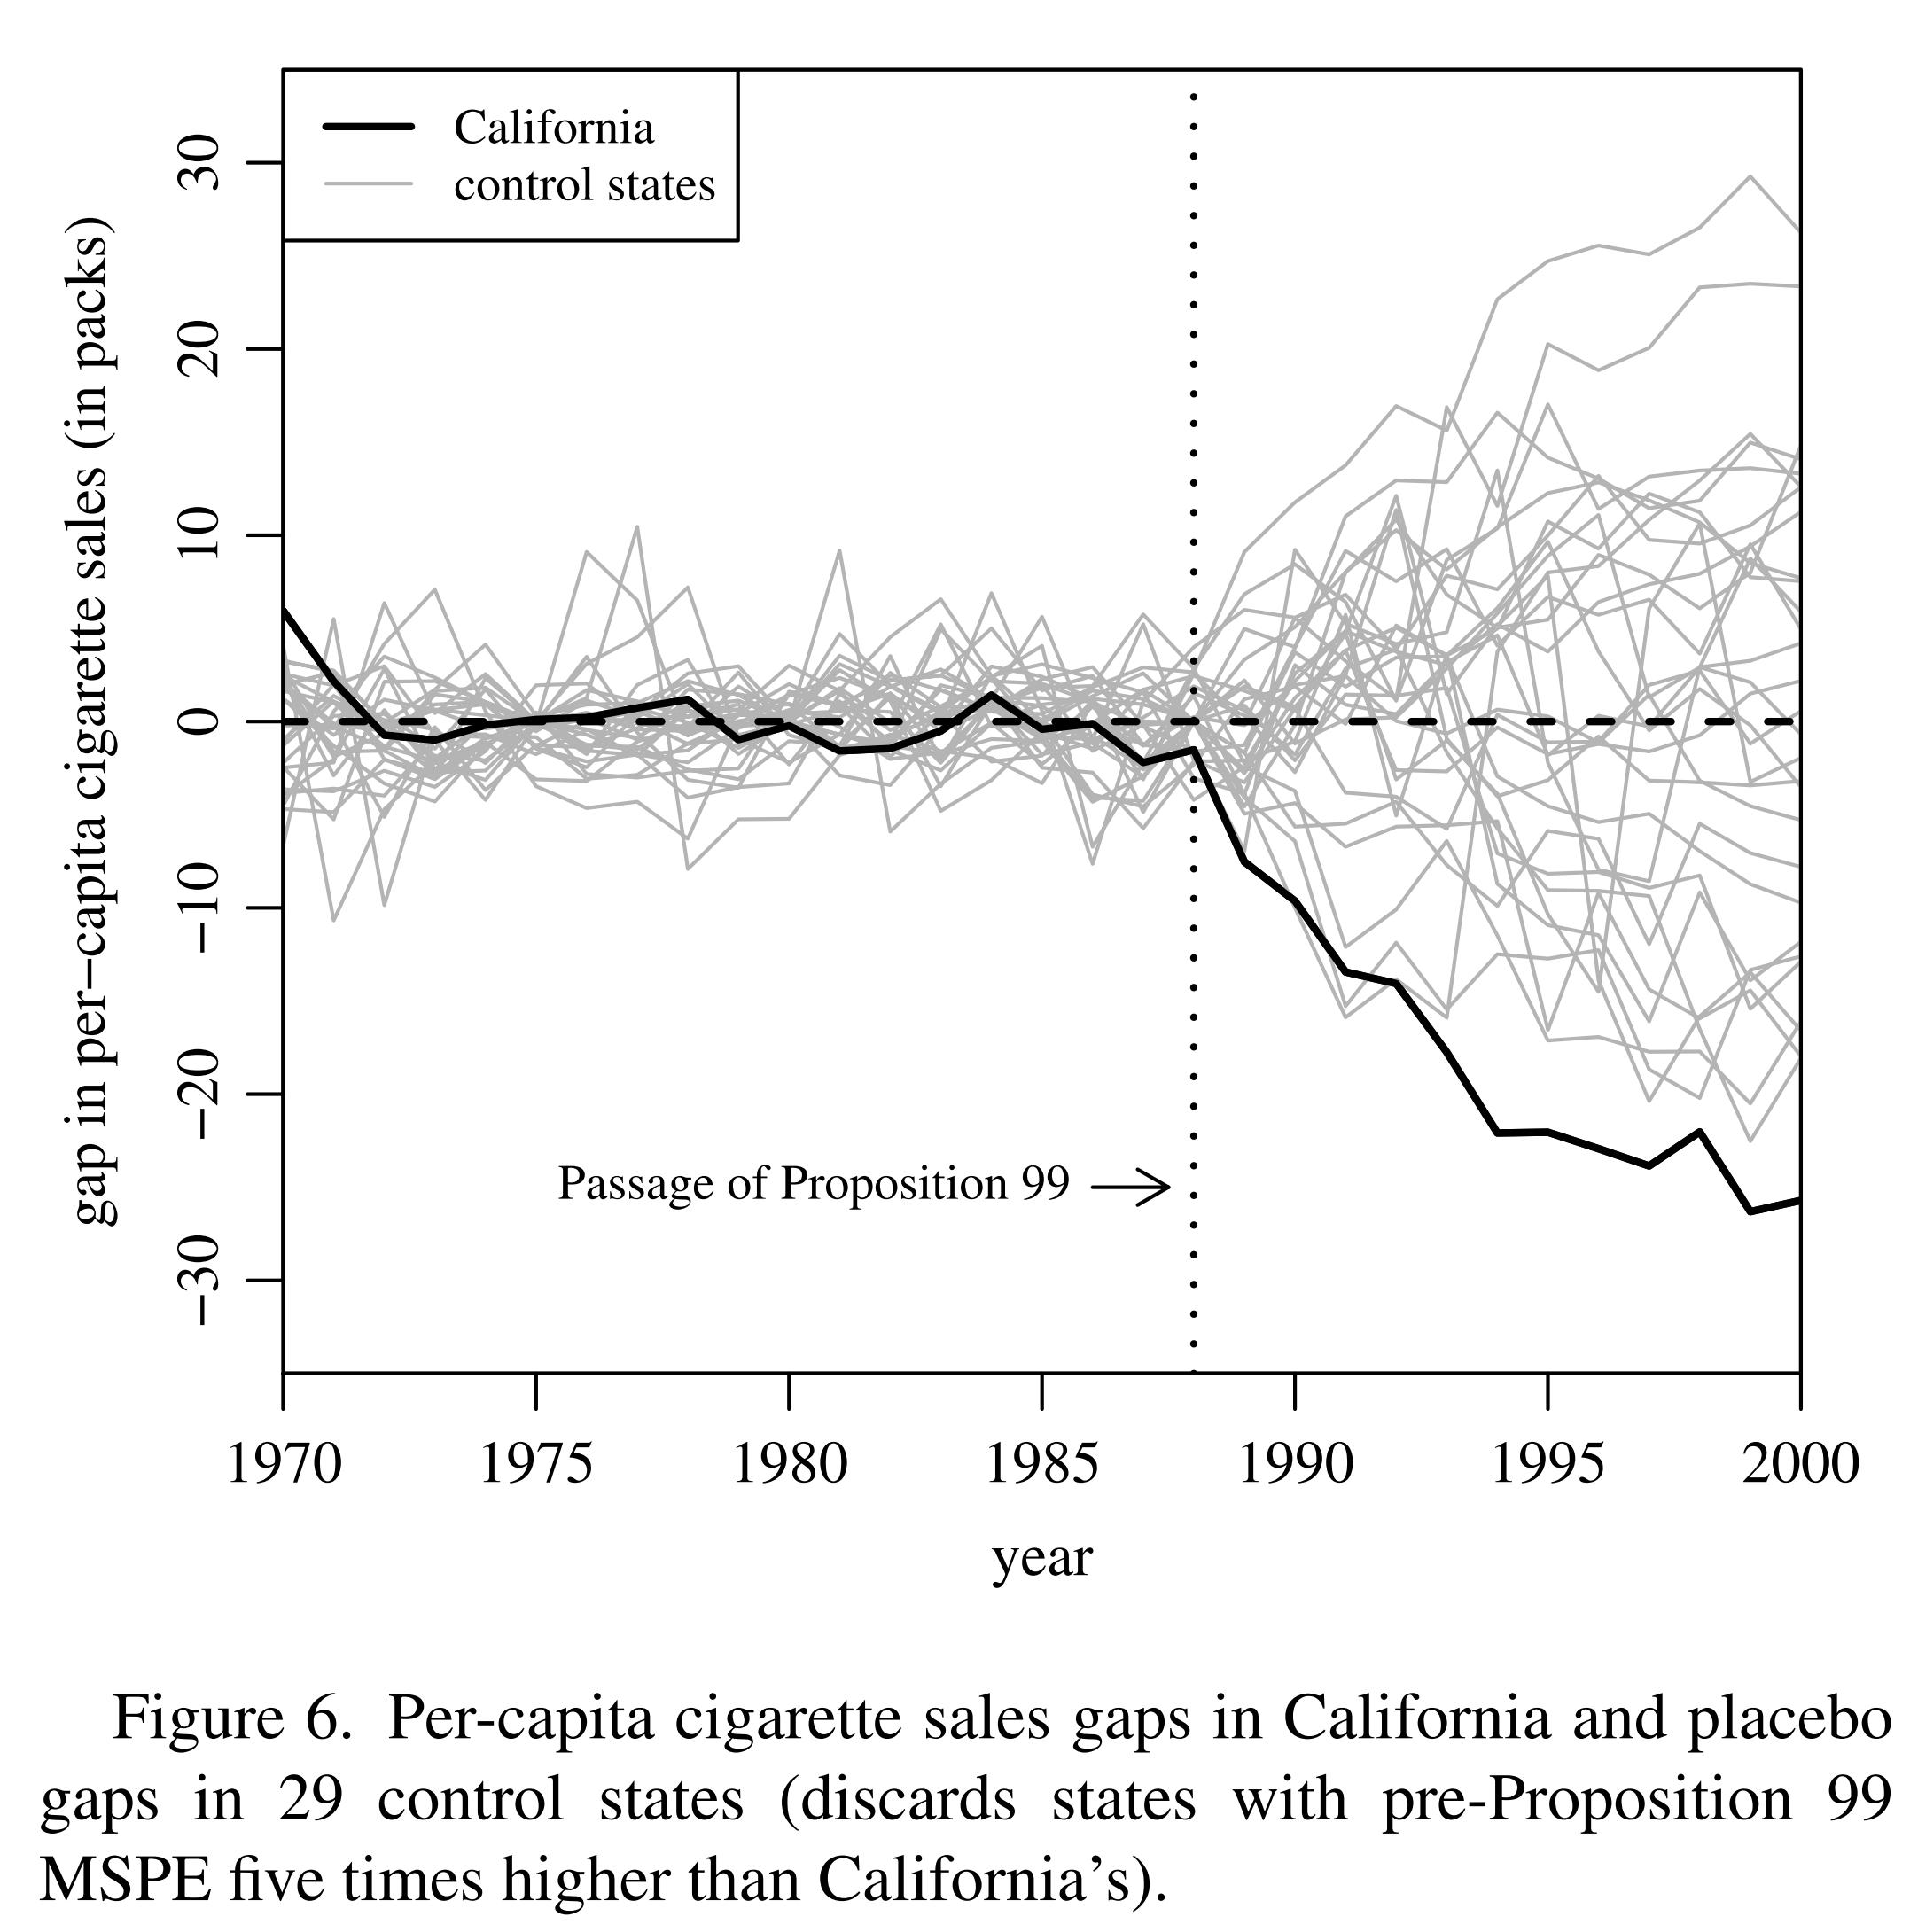
\includegraphics{figure/sc_f6.jpg}}
		%\includegraphics{sc-5.jpg}
	\end{figure}
\end{center}
\end{frame}




\begin{frame}{Statistical Inference of SC}{Standardized p-value}
	\begin{itemize}
		
	\item \textbf{Method 2:}
				\vspace{0.2cm}
			\begin{itemize}
		\item We can also calculate p-value by taking pre-treatment matching quality into account: 
		
	\begin{equation*}
		p^{std}_{1t}=\dfrac{\sum^{J+1}_{i=2}\mathbf{1}\{\dfrac{\hat{\alpha}_{it}}{RMSPE^{pre}_{i}} \geq   \dfrac{\hat{\alpha}_{1t}}{RMSPE^{pre}_{1}}\}}{J}
	\end{equation*}
		
		
		\begin{equation*}
			RMSPE^{pre}_{i}= 	\sqrt{\dfrac{			\sum^{T_{0}}_{t=1}(Y_{it} - Y^{SC}_{it})^{2}}{T_{0}}}
		\end{equation*}
		
			\end{itemize}
	\end{itemize}
\end{frame}



\begin{frame}{Statistical Inference of SC}{RMSPE Ratio Test}
	\begin{itemize}
		\item \textbf{Method 3:}
		\vspace{0.2cm}
		\begin{itemize}
			\item We can evaluate the significance by comparing the ratio of post/pre-treatment RMSPE:
			
			\begin{equation*}
				p^{ratio}_{1}=\dfrac{\sum^{J+1}_{i=2}\mathbf{1}\{\dfrac{RMSPE^{post}_{i}}{RMSPE^{pre}_{i}} \geq \dfrac{RMSPE^{post}_{1}}{RMSPE^{pre}_{1}}\}}{J}
			\end{equation*}
			
			\begin{equation*}
				RMSPE^{post}_{i}= \sqrt{\dfrac{\sum^{T}_{t=T_{0}+1}(Y_{it} - Y^{SC}_{it})^{2}}{T-T_{0}}}
			\end{equation*}
			
			\item This method evaluates whether the treatment effect is large relative to the pre-treatment fit
					\vspace{0.2cm}
			\item A large ratio indicates that the post-treatment deviation is substantial compared to pre-treatment matching quality
		\end{itemize}
	\end{itemize}
\end{frame}

\title[]  
{STATA Example}


\author 
{}

%\institute{Institute of Economics, Academia Sinica  \\ Econ, NTU}
%\institute{Institute of Economics, Academia Sinica  \\ IMES/IDAS, NCCU}
\institute{}

%\author 
%{楊子霆 \\ 中研院經濟所}

%\institute 
%{中正大學國際經濟專題研討}




\date
{}


\begin{frame}{}
	\titlepage
\end{frame}


\begin{frame}{STATA Example: Kim (2022)}{The Effect of Paid Leave on Fertility}
Brian Kim (2022), \textbf{``The Effect of Paid Leave on Fertility: Evidence from New York''}, Master Thesis
\begin{itemize}
	\vspace{0.2cm}
	\item The study examines the effect of paid parental leave on fertility rates in New York using synthetic control analysis.
	\vspace{0.2cm}
	\item Synthetic control method is used to estimate the counterfactual fertility rates in the absence of the policy.
\end{itemize}
\end{frame}




\begin{frame}{Overview}{Program and Data}
	\begin{itemize}
		\item See SCM.do
		\vspace{0.2cm}
		\item Use fert\_rate\_synth.csv
		\vspace{0.2cm}
		\item Install the following ado files:
		\begin{itemize}
			\vspace{0.2cm}
			\item synth2.ado 
		
			
		\end{itemize}
		
	\end{itemize}
\end{frame}





\begin{frame}[fragile]{Overview}{Stata Commends}
\begin{itemize}

	\item \texttt{synth2}:
	\vspace{0.2cm}
	\begin{itemize}
		\item Can be used for \textbf{single treated unit}
		\vspace{0.2cm}
		\item Supports \textbf{placebo tests} and allows for the exclusion of control units with poor pre-treatment fit.
		\vspace{0.2cm}
		\item Provides options for \textbf{graphing and post-processing}, including the ability to save and export results as graphs.
		\vspace{0.2cm}
		\item Offers robust options for conducting \textbf{statistical inference}, including the ability to calculate p-values.
	\end{itemize}
\end{itemize}
\end{frame}




\begin{frame}[fragile]{Overview}{Data}	
	\begin{itemize}
		
		
		\item This project examines the effect of paid-parental leave on fertility
					\vspace{0.2cm}		
		\begin{itemize}
			\item New York implements paid-parental leave in 2018
			\vspace{0.2cm}		
		\end{itemize}
		
		\item Use synthetic control method to evaluate its impact		
		\vspace{0.2cm}		
		\item The dataset contains state-level fertility rate and other demographic variables from 2007-2019
		\vspace{0.2cm}
		
		
		\begin{itemize}	
			\vspace{0.2cm}	
			\item \textbf{fert:} Fertility rate, which is the outcome variable
			\vspace{0.2cm}
			\item \textbf{year:} This is the year and is the time variable
			\vspace{0.2cm}
			\item \textbf{state:} This is an id number for each state and provides the individual identifier in this panel data context
		\end{itemize}
		
	\end{itemize}
	
	
	
	
\end{frame}



\begin{frame}[fragile]{Install package}
\begin{lstlisting}
ssc install synth2
\end{lstlisting}
	
\begin{lstlisting}
net install gr_postproduce, from("https://raw.githubusercontent.com/DiegoCiccia/StataPostProduce/main") replace
\end{lstlisting}
	
\begin{itemize}
	\item \texttt{synth2} is used for synthetic control analysis, while \texttt{gr\_postproduce} helps with post-processing and customizing graphs.
\end{itemize}	
\end{frame}






\begin{frame}[fragile]{Step 0: Data Preparation}
\begin{itemize}
	\item Assign labels to states based on their IPUMS codes. This allows us to translate numeric codes into meaningful state names in our analysis:
	\vspace{0.2cm}
\begin{lstlisting}
label define state_labels 1 "Alabama" 2 "Alaska" ...
label values ipums state_labels
\end{lstlisting}
	\item The \texttt{label define} command creates a mapping between the state codes and their names, while \texttt{label values} applies this label to the \texttt{ipums} variable.
	\vspace{0.2cm}
	\item This step ensures that state names are displayed in the results instead of numeric codes, making interpretation easier.
\end{itemize}
\end{frame}





\begin{frame}[fragile]{Step 1: Setting Up Panel Data}
\begin{itemize}
	\item Declare the data as panel data:
\begin{lstlisting}
xtset ipums year
\end{lstlisting}
	\item The \textbf{xtset} command declares \texttt{ipums} as the panel variable (state) and `year` as the time variable.

\end{itemize}
\end{frame}


\begin{frame}[fragile]{Step 2: SC Estimation}
\begin{itemize}
	\item Syntax:	
\begin{lstlisting}
synth2 depvar predictorvars, trunit(#) trperiod(#)
\end{lstlisting}
	
	\item \textbf{depvar}: the outcome variable (Y)
	\vspace{0.2cm}
	\item \textbf{predictorvars}: the list of predictor variables (Z)
	\vspace{0.2cm}
	\item By default, all predictor variables are \textbf{averaged over the entire pre-treatment period}
\end{itemize}


\end{frame}


\begin{frame}[fragile]{Step 2: SC Estimation}
\begin{itemize}
	\item Run the synthetic control method using `synth2`:
\begin{lstlisting}
synth2 fert avginc black educattain white asian_pi hisp ///
fert(2017) fert(2016) fert(2015) fert(2014) fert(2013) fert(2012) ///
fert(2011) fert(2010) fert(2009) fert(2008) fert(2007), ///
trunit(36) trperiod(2018) xperiod(2007(1)2017)
\end{lstlisting}
\vspace{0.2cm}
\item \textbf{fert(2017)}: the value of the variable \textbf{fert} in 2017 is entered as a predictor
\vspace{0.2cm}
\item \textbf{xperiod(2007(1)2017)}: periods over 2007-2017 the covariates specified in predictorvars are averaged
\end{itemize}
\end{frame}


\begin{frame}{Results: Unit Weights for SC}
\begin{itemize}
	\item Top 3 countries that consist synthetic China
	\begin{itemize}
		\vspace{0.2cm}
		\item New Hampshire: 23.1\%
		\vspace{0.2cm}
		\item Kansas: 23.1\%
		\vspace{0.2cm}
		\item Massachusetts: 15.8\%		
	\end{itemize}
	
	
\end{itemize}
\end{frame}


\begin{frame}[fragile]{Step 3: Statistical Inference}
\begin{itemize}
\item Conduct placebo tests using the `synth2` command:
\begin{lstlisting}
synth2 fert fert(2017) fert(2016) fert(2015) fert(2014) ///
fert(2013) fert(2012) fert(2011) fert(2010) fert(2009) ///
fert(2008) fert(2007), trunit(36) trperiod(2018) ///
xperiod(2007(1)2017) placebo(unit cutoff(2))
\end{lstlisting}
	\item The \textbf{placebo(unit cutoff(2))} option excludes states where pre-treatment MSPE is twice that of the treated unit (New York).
\end{itemize}
\end{frame}




\begin{frame}[fragile]{Graphing Results}
\begin{itemize}
	\item Generate a data frame for storing results and save graphs:
\begin{lstlisting}
synth2 fert fert(2017) fert(2016) fert(2015) fert(2014) ///
fert(2013) fert(2012) fert(2011) fert(2010) fert(2009) ///
fert(2008) fert(2007), trunit(36) trperiod(2018) ///
xperiod(2007(1)2017) frame(ny_fert) savegraph(ny_fert, replace)
\end{lstlisting}

\end{itemize}
\end{frame}


\begin{frame}[fragile]{Post-Processing Graphs}
\begin{itemize}
	\item Enhance graph appearance:
\vspace{0.2cm}
\begin{lstlisting}
graph use "$pic\ny_fert_eff.gph"

gr_postproduce ny_fert_eff, ///
title("The Effect of Paid Leave on Fertility") ///
ytitle("Effects") xtitle("Year")
graph export "$pic\ny_fert_eff.png"
\end{lstlisting}
\item Post-process and export the graph with \textbf{gr\_postproduce}
\end{itemize}
\end{frame}


\begin{frame}[fragile]{Working with Frames}
\begin{itemize}
	\item Switch to the results frame:
	\vspace{0.2cm}
\begin{lstlisting}
frame change ny_fert
\end{lstlisting}
	\vspace{0.2cm}
	\item Export results to CSV:
	\vspace{0.2cm}
\begin{lstlisting}
export delimited "$rawdata\ny_fert.csv",replace
\end{lstlisting}
	\vspace{0.2cm}
	\item Clear all frames and return to default:
	\vspace{0.2cm}
\begin{lstlisting}
frames reset
\end{lstlisting}
\end{itemize}

\end{frame}



\title[]  
{R Example}


\author 
{}

%\institute{Institute of Economics, Academia Sinica  \\ Econ, NTU}
%\institute{Institute of Economics, Academia Sinica  \\ IMES/IDAS, NCCU}
\institute{}

%\author 
%{楊子霆 \\ 中研院經濟所}

%\institute 
%{中正大學國際經濟專題研討}




\date
{}


\begin{frame}{}
\titlepage
\end{frame}




\begin{frame}{Overview}{Program and Data}
\begin{itemize}
	\item See SCM.R
	\vspace{0.2cm}
	\item Use fert\_rate\_synth.csv
	\vspace{0.2cm}
	\item Install the following package:
	\begin{itemize}
		\vspace{0.2cm}
		\item tidysynth 
		
		
	\end{itemize}
	
\end{itemize}
\end{frame}



\begin{frame}[fragile]{Step 0: Install package}
\begin{itemize}
	\item Install required packages:
	\vspace{0.2cm}
\begin{lstlisting}
install.packages("tidysynth")


library(tidyverse)
library(tidysynth)
library(haven)
\end{lstlisting}
	\item \textbf{tidysynth}: Main package for synthetic control
	\item \textbf{tidyverse}: Data manipulation and visualization
	\item \textbf{haven}: Reading various data formats
\end{itemize}
\end{frame}

\begin{frame}[fragile]{Step 0: Data Preparation}
\begin{itemize}
\item Read and clean the data:
\vspace{0.2cm}
\begin{lstlisting}
fert_data <- fert_data_raw %>%
# Drop specific states and years
filter(!(ipums %in% c(6, 34, 44, 53))) %>%  
filter(year < 2020) %>%
mutate(
avginc = Personal.income/Population
) %>%
select(-statecode)
\end{lstlisting}
\vspace{0.2cm}
\item Key steps:
\begin{itemize}
	\item Drop CA, NJ, RI, WA (states with similar policies)
	\item Remove data after 2020
	\item Calculate average income
	\item Remove unnecessary columns
\end{itemize}
\end{itemize}
\end{frame}

\begin{frame}[fragile]{Step 2: SC Estimation}
\begin{itemize}
\item Initialize synthetic control:
\vspace{0.2cm}
\begin{lstlisting}
synth_fert <- fert_data %>%
synthetic_control(
outcome = fert,
unit = state,
time = year,
i_unit = "New York",
i_time = 2018,
generate_placebos = TRUE
)
\end{lstlisting}
\vspace{0.2cm}
\item Parameters:
\begin{itemize}
\item \texttt{outcome}: Fertility rate
\item \texttt{unit}: State identifier
\item \texttt{i\_unit}: Treated unit (New York)
\item \texttt{i\_time}: Treatment year (2018)
\end{itemize}
\end{itemize}
\end{frame}

\begin{frame}[fragile]{Step 2: SC Estimation}{Add Predictors}
\begin{itemize}
\item Add demographic predictors:
\vspace{0.2cm}
\begin{lstlisting}
generate_predictor(
time_window = 2007:2017,
avg_income = mean(avginc, na.rm = TRUE),
black_pop = mean(black, na.rm = TRUE),
educ_attain = mean(educattain, na.rm = TRUE),
white_pop = mean(white, na.rm = TRUE),
asian_pop = mean(asian_pi, na.rm = TRUE),
hisp_pop = mean(hisp, na.rm = TRUE)
)
\end{lstlisting}
\item Takes average of demographics over 2007-2017
\item Handles missing values with \texttt{na.rm = TRUE}
\end{itemize}
\end{frame}

\begin{frame}[fragile]{Step 2: SC Estimation}{Add Predictors}
\begin{itemize}
\item Add lagged fertility rates:
\vspace{0.2cm}
\begin{lstlisting}
generate_predictor(
time_window = 2017,
fert_2017 = fert
) %>%
generate_predictor(
time_window = 2016,
fert_2016 = fert
)
# ... (similar for other years)
\end{lstlisting}
\item Adds fertility rates for each year from 2007-2017
\item Each year added separately for flexibility
\end{itemize}
\end{frame}

\begin{frame}[fragile]{Step 2: SC Estimation}{Weight Generation}
\begin{itemize}
\item Generate synthetic control weights:
\vspace{0.2cm}
\begin{lstlisting}
 # Generate weights using default optimization parameters
generate_weights(optimization_window = 2007:2017) %>%
generate_control()
\end{lstlisting}
\item Parameters:
\begin{itemize}
\item \texttt{optimization\_window}: Time period for weight calculation
%\item \texttt{margin\_ipop}: Convergence margin
%\item \texttt{sigf\_ipop}: Significant figures in optimization
%\item \texttt{bound\_ipop}: Optimization boundary
\end{itemize}
\end{itemize}
\end{frame}

\begin{frame}[fragile]{Graphing Results}
\begin{itemize}
\item Generate and display plots:
\vspace{0.2cm}
\begin{lstlisting}
plot_trends <- synth_fert %>%
plot_trends() +
labs(
title = "Fertility Trends: NY vs Synthetic Control",
y = "Fertility Rate",
x = "Year"
)

print(plot_trends)  
ggsave("synth_fert.png", plot = plot_trends)
\end{lstlisting}
\item Three types of plots:
\begin{itemize}
\item Trends plot: Actual vs synthetic
\item Differences plot: Gap analysis
\item Placebos plot: Statistical inference
\end{itemize}
\end{itemize}
\end{frame}


\begin{frame}[fragile]{Graphing Results}
\begin{itemize}
	\item Generate and display difference plot:
	\vspace{0.2cm}
\begin{lstlisting}
plot_differences <- synth_fert %>%
plot_differences() +
labs(
title = "Gap in Fertility Rates",
y = "Difference in Fertility Rate",
x = "Year"
)

print(plot_differences)
ggsave("synth_fert_differences.png", 
plot = plot_differences)
\end{lstlisting}
	\item Gap Analysis Features:
	\begin{itemize}
		\item Shows treatment effect over time
		\item Zero line indicates no effect
		\item Negative values show fertility decrease
		\item Helps identify pre-treatment fit quality
	\end{itemize}
\end{itemize}
\end{frame}

\begin{frame}[fragile]{Graphing Results}
\begin{itemize}
\item Generate and display placebo plot:
\vspace{0.2cm}
\begin{lstlisting}
plot_placebos <- synth_fert %>%
plot_placebos() +
labs(
title = "Placebo Tests",
y = "Gap in Fertility Rate",
x = "Year"
)

print(plot_placebos)
ggsave("synth_fert_placebos.png", 
plot = plot_placebos)
\end{lstlisting}
\item Placebo Test Features:
\begin{itemize}
	\item Shows treatment effects for all states
	\item Treated unit highlighted
	\item Provides visual inference
	\item Helps assess significance of results
\end{itemize}
\end{itemize}
\end{frame}

\begin{frame}[fragile]{Results Export}
\begin{itemize}
\item Save results and tables:
\vspace{0.2cm}
\begin{lstlisting}
summary_tables <- synth_fert %>%
grab_synthetic_control()
predictor_balance <- synth_fert %>%
grab_balance_table()


write_csv(summary_tables, 
file.path(workdata, "ny_fert_results.csv"))
write_csv(predictor_balance, 
file.path(workdata, "ny_fert_balance.csv"))
\end{lstlisting}
\item Exports:
\begin{itemize}
\item Synthetic control results
\item Predictor balance tables
\end{itemize}
\end{itemize}
\end{frame}









\title[]  
{Practical Issues}


\author 
{}

%\institute{Institute of Economics, Academia Sinica  \\ Econ, NTU}
%\institute{Institute of Economics, Academia Sinica  \\ IMES/IDAS, NCCU}
\institute{}

%\author 
%{楊子霆 \\ 中研院經濟所}

%\institute 
%{中正大學國際經濟專題研討}




\date
{}


\begin{frame}{}
	\titlepage
\end{frame}




\begin{frame}{Practical Issues with SC}{Computation Time}
	\begin{itemize}
		\item The STATA command \texttt{synth} implements an optimization procedure to select the optimal $W^*$ for each treated $i$
		\vspace{0.2cm}
		\item The optimization scheme suffers from a curse of dimensionality
		\vspace{0.2cm}
		\begin{itemize}
			\item Lots of non-treated units increase the number of potential $W$'s
		\end{itemize}
		\vspace{0.2cm}
		\item One way to reduce computation time is to only use non-treated units that are similar to treated units
		\begin{itemize}
			\vspace{0.2cm}
			\item It also improve match quality
			
			%Also helps fit the assumption that they follow the same factor process
		\end{itemize}
	\end{itemize}
\end{frame}



%\begin{frame}{Practical Issues with SC}{Computation Time}
%	\begin{itemize}
%		\item Many of the inference methods require the use of a large number of placebo treatment groups
%		\begin{itemize}
%			\vspace{0.2cm}
%			\item Single treated problems only require placebo treated \textbf{units}, multiple treated problems require placebo \textbf{groups}
%		\end{itemize}
%		\vspace{0.2cm}
%		\item Thus, it may be computationally infeasible to implement the Cavallo et. al (2013) method with a large $G$ and $J$
%		%\begin{itemize}
%		%\vspace{0.2cm}
%		%\item Limit the number of placebo treatment groups to 5,000
%		
%		%My advice: Limit yourself to a maximum of 5,000 placebo treatment groups
%		%\end{itemize}
%	\end{itemize}
%\end{frame}






\begin{frame}{Practical Issues with SC}{Length of Pre-treatment Period}
	\begin{itemize}
		\item For the SC estimator to estimate the parameter of interest, the ``\textbf{pre-treatment period must be large relative to the scale of the transitory shocks}"
		\begin{itemize}
			\vspace{0.2cm}
			\item This is ambiguous, and it is unclear how to test necessary conditions of whether this holds in the data
		\end{itemize}
	\end{itemize}
\end{frame}



\begin{frame}{Suggested Readings}
	\begin{itemize} 
		\item Chapter 10, Causal Inference: The Mixtape
		\vspace{0.2cm}
		\item Abadie, A. (2019). Using synthetic controls: Feasibility, data requirements, and methodological aspects. Journal of Economic Literature.
	\end{itemize}
\end{frame}









\end{document} 